\chapter{Resultados y discusión}
En este capítulo se presentan los resultados obtenidos de las simulaciones de transmisión de calor por conducción de un sistema TPV de un nano-espaciador y
radiación por campo cercano entre dos placas paralelas a 800°C el emisor y 25°C la célula. A su vez se representa las relaciones entre la potencia radiada vs la potencia conducida por cantidad de espaciadores y por distancia de separación en un sistema de emisor y célula de 1cm2.
\begin{itemize}
	\item Primero se comprueba si el procedimiento de extracción de datos de la simulación de transmisión de calor por conducción en CFD es adecuado y no presenta un error relativo significativo respecto a la teoría.
	\item Se presentan los resultados de las simulaciones de transmisión de calor por conducción y por radiación de campo cercano para diferentes combinaciones de materiales de emisor y célula, y la relación entre ambas simulaciones.
	\item Se estudia el número mínimo de espaciadores necesarios para soportar la carga de los emisores.
	\item Por último, se presentan los resultados de usar un nano-espaciador de $Si$ en vez de $SiO_2$ para emisores de $Si$ y $SS$.
\end{itemize}
%% COMPROBACIÓN DEL PROCEDIMIENTO DE EXTRACCIÓN DE RESULTADOS DE CFD
\section{Comprobación del procedimiento de extracción de resultados de CFD}
El procedimiento de extracción de resultados de CFD está definido en el punto \ref{it:extraerResCFD} del capítulo \ref{chapter:Metodos} y para su comprobación se procede a realizar una simulación en CFD donde el emisor y la célula son de $Si$ y el nano-espaciador de $SiO_2$ con las características constantes a 25\textdegree C, con la base cuadrada de 1 $mm^2$ y la altura del nano-espaciador a unos 1000nm, todo con la escalas correspondientes aplicadas.\\\\
La conductividad térmica ($\sigma$) del $Si$ es 182.977 W/m\textdegree C y la del $SiO_2$ es 1.30067 W/m\textdegree C ambas a 25\textdegree C. De la simulación se extrae que el flujo de calor del sistema y la temperatura media máxima y mínima de las superficies de contacto del nano-espaciador con los otros componentes del sistema.\\\\
La temperatura media máxima del nano-espaciador es 792.601\textdegree C, la temperatura media mínima del nano-espaciador es 32.3903\textdegree C y el flujo de calor es 0.00889793 W. Con los resultados de las temperaturas medias del nano-espaciador se obtiene un flujo de calor teórico de 0.00889905 W, obteniéndose un error relativo aproximado del 0.0126\%, por lo tanto el procedimiento es apropiado para la obtención de los resultados de las simulaciones de transmisión de calor por conducción.
%%% SIMULACIONES DE TRANSMISIÓN DE CALOR POR CONDUCCIÓN EN CFD
\section{Resultados de las simulaciones para una TPV de Si-SiO2-Si}
A continuación se estudian los efectos de la resistencia de contacto y la porosidad sobre un sistema sencillo compuesto por un emisor de $Si$ de 1 $mm$ lado y 0.2 $mm$ de altura con la cara superior a 800 \textdegree C, un nano-espaciador de 3 $\mu m$ de lado y una célula de $Si$ de las mismas dimensiones que el emisor con la cara inferior a 25\textdegree C.
\subsection{Efectos de la resistencia de contacto sobre la conducción}
La resistencia de contacto usada es de unos $4\cdot 10^{-6} \ m^2 K/W$ \cite{nf_TPV_Pillars_SiO2} que es aplicada a la superficie superior del nano-espaciador que entra en contacto con la superficie inferior del emisor, solo se considera en dicha superficie porque el nano-espaciador será depositado sobre la superficie de la célula en la fase de fabricación.
\begin{figure}[H]
	\centering
	\begin{subfigure}[b]{0.49\textwidth}
		\centering
		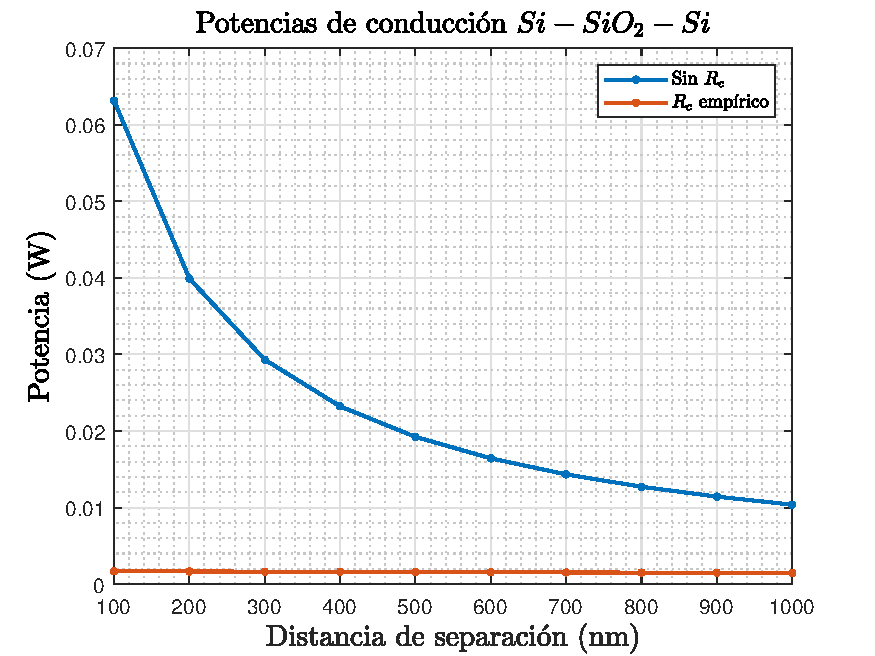
\includegraphics[width=1.0\textwidth]{figuras/Resultados/conduccion/pdf/Prc_SiSiO2Si.pdf}
		\caption{Efecto de la $R_c$}
		\label{fig:Prc_SiSiO2Si}
	\end{subfigure}
	\hfill
	\begin{subfigure}[b]{0.49\textwidth}
		\centering
		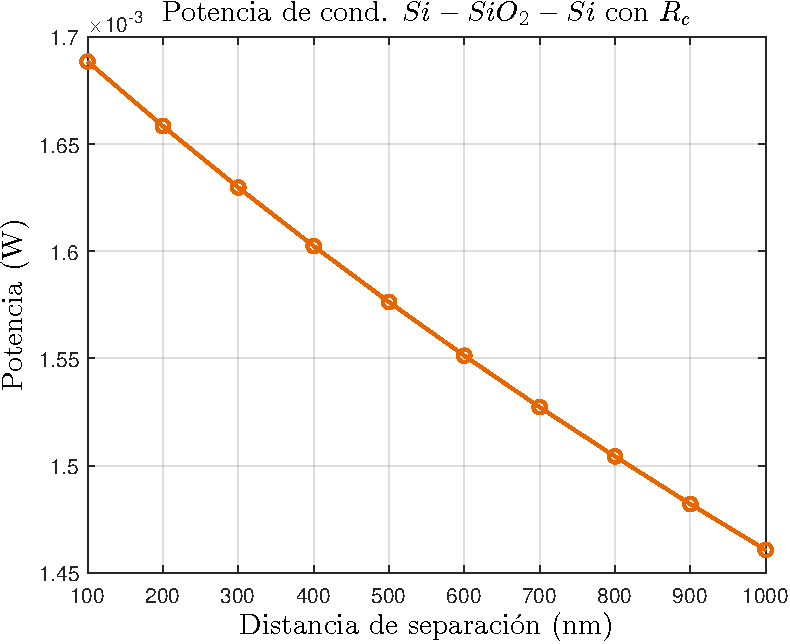
\includegraphics[width=1.0\textwidth]{figuras/Resultados/conduccion/pdf/Prc2_SiSiO2Si.pdf}
		\caption{Efecto de la $R_c$ por separado}
		\label{fig:Prc2_SiSiO2Si}
	\end{subfigure}
	\caption[Efectos de la resistencia de contacto sobre el flujo de calor por conducción]{Gráficas de los efectos de la porosidad y de la resistencia de contacto sobre el flujo de calor por conducción. (\subref{fig:Prc_SiSiO2Si},\subref{fig:Prc2_SiSiO2Si}) Comparación de la potencia conducida de un nano-espaciador sin $R_c$ y con $R_c$ en un mismo eje (\subref{fig:Prc_SiSiO2Si}) y en dos ejes (\subref{fig:Prc2_SiSiO2Si})}
	\label{fig:PcondRc_SiSiO2Si}
\end{figure}
Para un área de 9$\mu m^2$ la resistencia de contacto total es aproximadamente de $444.44\cdot 10^3 \ K/W$ comparada con los $85.43\cdot 10^3 \ K/W$ de la mayor resistencia que presenta el nano-espaciador con 1000nm de altura a 25\textdegree C es al menos 5 veces más grande, por lo cual, como se observa en las figuras \ref{fig:Prc_SiSiO2Si} y \ref{fig:Prc2_SiSiO2Si} la resistencia de contacto constante domina sobre la resistencia del nano-espaciador dando así la forma aproximada de una recta porque la mayor caída de temperatura se dá en la superficie de contacto, evitando que aumente la temperatura del nano-espaciador variando menos su resistencia térmica, por ende, dependerá principalmente de la altura del nano-espaciador.
\begin{figure}[H]
	\centering
		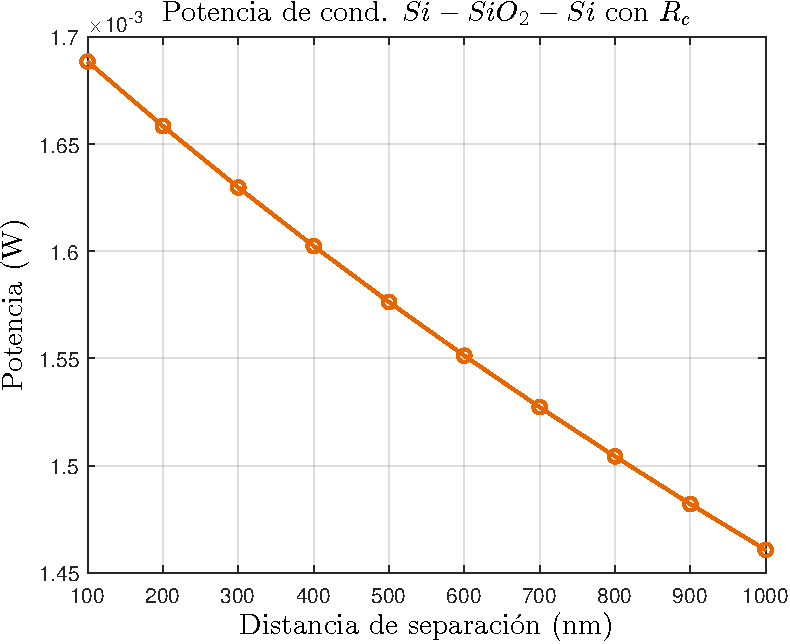
\includegraphics[width=0.49\textwidth]{figuras/Resultados/conduccion/pdf/relPrc_SiSiO2Si.pdf}
		\caption{Relación de la potencia de la $R_c$ respecto a sin $R_c$}
	\label{fig:relPrc_SiSiO2Si}
\end{figure}
La disminución de flujo de calor por conducción es significativa para todos los casos, siendo la potencia de conducción con $R_c$ variando aproximadamente entre un 3\% y un 14\% de la potencia sin $R_c$, lo que implica una disminución de conducción de unos 97\% y 85\%.\\\\
Hay que tomar en cuenta que la resistencia de contacto en la realidad no es constante con la temperatura a diferencia de las simulaciones en CFD donde la $R_c$ es constante, pero sirve para tener una primera idea de su importancia en la eliminación de la transferencia de calor por conducción.
\subsection{Efecto de la porosidad sobre la conducción}
\begin{figure}[H]
\centering
	\begin{subfigure}[b]{0.49\textwidth}
		\centering
		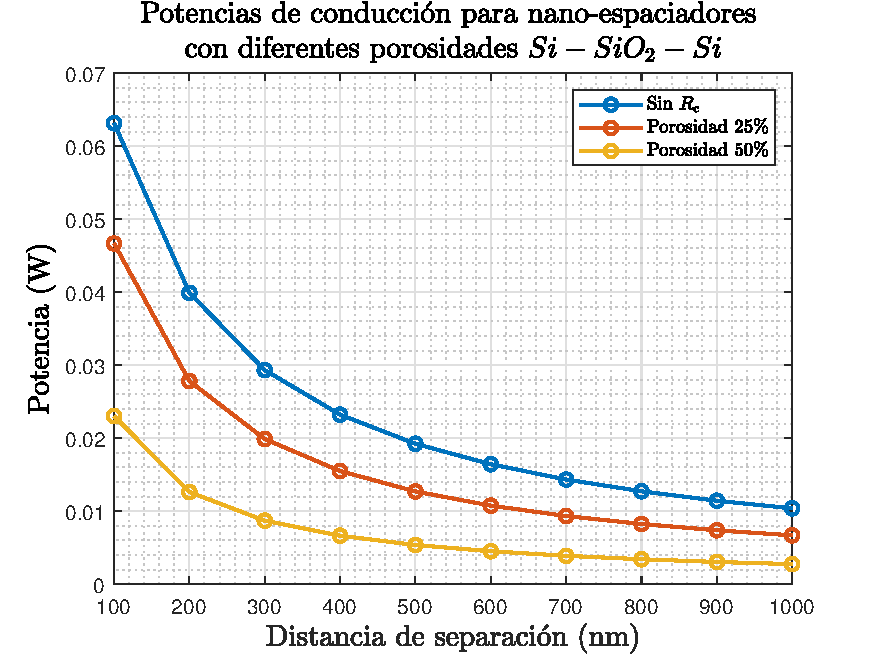
\includegraphics[width=1.0\textwidth]{figuras/Resultados/conduccion/pdf/Ppor_SiSiO2Si.pdf}
		\caption{Efecto de la Porosidad}
		\label{fig:Ppor_SiSiO2Si}
	\end{subfigure}
	\hfill
	\begin{subfigure}[b]{0.49\textwidth}
		\centering
		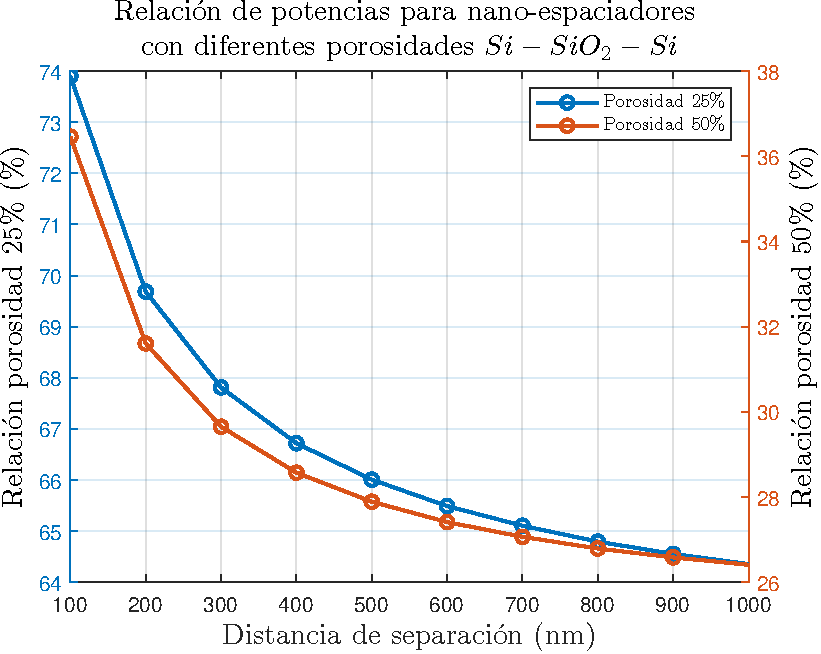
\includegraphics[width=1.0\textwidth]{figuras/Resultados/conduccion/pdf/relPpor_SiSiO2Si.pdf}
		\caption{Efecto de la Porosidad relativo}
		\label{fig:relPpor_SiSiO2Si}
	\end{subfigure}
	\caption[Efectos de la porosidad del nano-espaciador sobre el flujo de calor por conducción]{Gráficas de los efectos de la resistencia de contacto sobre el flujo de calor por conducción. (\subref{fig:Ppor_SiSiO2Si}) Efecto del grado de porosidad del $SiO_2$ sobre el flujo de calor por conducción para unos 0\%, 25\% y 50\%. (\subref{fig:relPpor_SiSiO2Si}) Relación de los efectos de la porosidad en la transmisión de calor por conducción respecto a la porosidad del 0\%.}
	\label{fig:PcondPor_SiSiO2Si}
\end{figure}
%% Ahora a comentar sobre las porosidades
Para diferentes porosidades la conductividad térmica varía, disminuyendo con el aumento del grado de porosidad \cite{ThermalConductivity_SiO2_2018}, por este motivo la potencia de conducción disminuye para todas las alturas de nano-espaciador. La relación o conductividad térmica normalizada para una porosidad del 25\% y 50\% son respectivamente 0.64 y 0.25 veces la conductividad térmica del material \cite{ThermalConductivity_SiO2_2018}.\\\\
Como se puede observar en las figuras \ref{fig:Prc_SiSiO2Si} y \ref{fig:Prc2_SiSiO2Si} las relaciones de potencia no se cumplen completamente porque la temperatura en todo el nano-espaciador no es la misma lo que produce que la conductividad térmica a lo largo del espaciador sea distinta. Por tal motivo, al disminuir la altura del nano-espaciador aumenta la relación porque aumenta el gradiente de temperatura.\\\\
Utilizando la aplicación \textbf{Curve Fitting} de MATLAB se obtiene un modelo matemático que relaciona la potencia de conducción respecto a la altura del nano-espaciador ($d$) y la porosidad del material del nano-espaciador ($\rho$), como se muestra en la ecuación \eqref{eq:Pcond_d_p} donde $d$ es en nanómetros.
\begin{equation}
P(d,\rho)=\frac{  16.47\cdot \rho-11.03 }{d-106.80\cdot \rho +74.68}
\label{eq:Pcond_d_p}
\end{equation}
%% RAD Si-SiO2-Si
\subsection{Radiación de campo cercano}
Para la radiación por campo cercano se utiliza la \textbf{calculadora de campo cercano} para dos placas gruesas de $Si$ para varias separaciones entre ellas. La radiación monocromática o potencia de radiación monocromática aumenta con la disminución de la distancia de separación como lo indica el componente exponencial en la ecuación \eqref{eq:flujoEvasNF} de \cite{nfTPV_equations}, como se puede observar en la figura \ref{fig:rad_SiSi_ds}.
\begin{figure}[H]
	\centering
		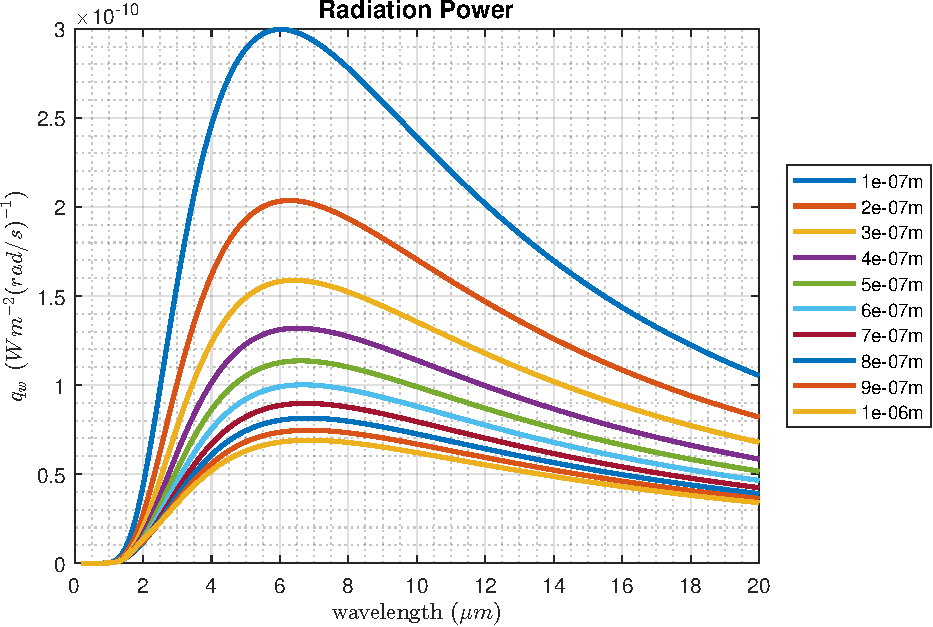
\includegraphics[width=0.7\textwidth]{figuras/Resultados/radiacion/SiSi_ds.pdf}
	\caption{Potencia de radiación monocromática para dos placas gruesas planas de $Si$ separadas diferentes distancias ($d$) en metros.}
	\label{fig:rad_SiSi_ds}
\end{figure}
Realizando la integral de la potencia monocromática en el rango de longitudes de onda con energías mayores a 1.1 eV, energía de banda del $Si$, se obtiene en promedio potencias del orden de $60 \ W/m^2$ (figura \ref{fig:prad_Eg11_SiSi}) a diferencia de todo el rango disponible, hasta las $\sim$20 $\mu m$, cuyo orden es de $10^4 \ W/m^2$ (figura \ref{fig:prad_full_SiSi}), desaprovechándose una gran cantidad de energía.
\begin{figure}[H]
	\centering
		\begin{subfigure}[b]{0.49\textwidth}
	\centering
		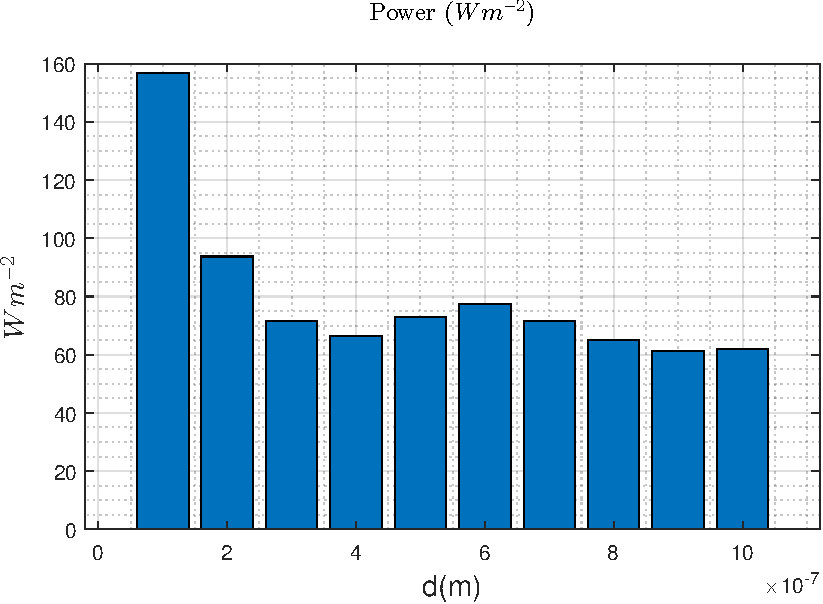
\includegraphics[width=1.00\textwidth]{figuras/Resultados/radiacion/p_11_SiSi.pdf}
	\caption{Potencia para energía mayor a 1.1 eV}
	\label{fig:prad_Eg11_SiSi}
\end{subfigure}
\hfill
\begin{subfigure}[b]{0.49\textwidth}
	\centering
		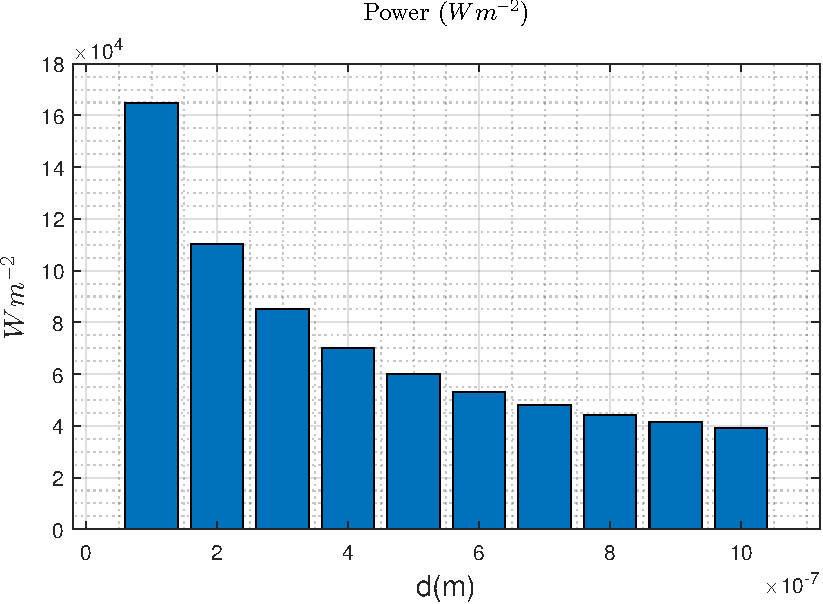
\includegraphics[width=1.00\textwidth]{figuras/Resultados/radiacion/p_full_SiSi.pdf}
	\caption{Potencia hasta las $\sim$20 $\mu m$}
	\label{fig:prad_full_SiSi}
\end{subfigure}
	\caption{(\subref{fig:prad_Eg11_SiSi}) Potencia por unidad de área transmitida por radiación por efecto de campo cercano para radiación monocromática de energía mayor a los 1.1 eV. (\subref{fig:prad_full_SiSi}) Potencia por unidad de área transmitida por radiación por efecto de campo cercano para radiación monocromática en todo el rango de longitudes de onda disponible.}
	\label{fig:prad_SiSi}
\end{figure}
Las potencias obtenidas para el rango de longitudes de onda mayor a la banda energética del $Si$ son muy pequeñas (figura \ref{fig:prad_Eg11_SiSi}), produciendo que no sea viable este sistema porque las pérdidas por conducción son demasiado grandes para 10 nano-espaciadores o más en el mejor caso con resistencia de contacto (figura \ref{fig:rel_SiSi11_Rc}).
\begin{figure}[H]
	\centering
\begin{subfigure}[b]{0.49\textwidth}
	\centering
		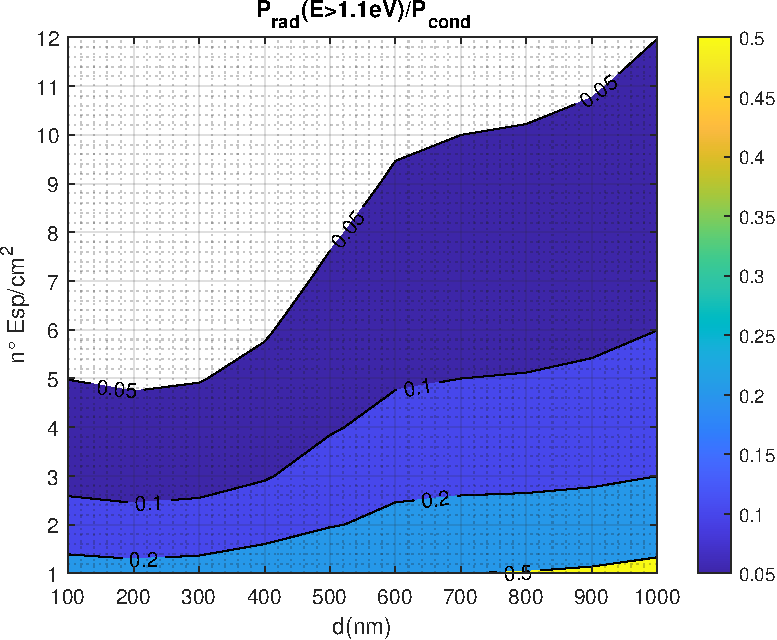
\includegraphics[width=1.00\textwidth]{figuras/Resultados/RelacionCondRad/rel_SiSi11.pdf}
	\caption{Relación de potencias para Eg$>$1.1 eV}
	\label{fig:rel_SiSi11}
\end{subfigure}
\hfill
\begin{subfigure}[b]{0.49\textwidth}
	\centering
		\includegraphics[width=1.00\textwidth]{figuras/Resultados/RelacionCondRad/rel_SiSi11_Rc.pdf}
	\caption{Relación de potencias para Eg$>$1.1 eV con $R_c$}
	\label{fig:rel_SiSi11_Rc}
\end{subfigure}
\caption{Relación de las potencias de radiación y conducción para un sistema TPV de 1$cm^2$ y célula de $Si$. (\subref{fig:rel_SiSi11}) Relación de las potencias para Eg$>$1.1 eV y si $R_c$. (\subref{fig:rel_SiSi11_Rc}) Relación de las potencias para Eg$>$1.1 eV y con $R_c$ \cite{nf_TPV_Pillars_SiO2}.}
	\label{fig:rels_SiSi11}
\end{figure}
Por lo tanto se procede a calcular la potencia por unidad de área de la radiación en el rango de longitudes de onda de energías mayor e igual a 0.7 eV (banda energética del $Ge$), utilizándose estos nuevos resultados para el resto de comparaciones para así tener una primera referencia de como será el sistema TPV en la realidad.
\begin{figure}[H]
	\centering
		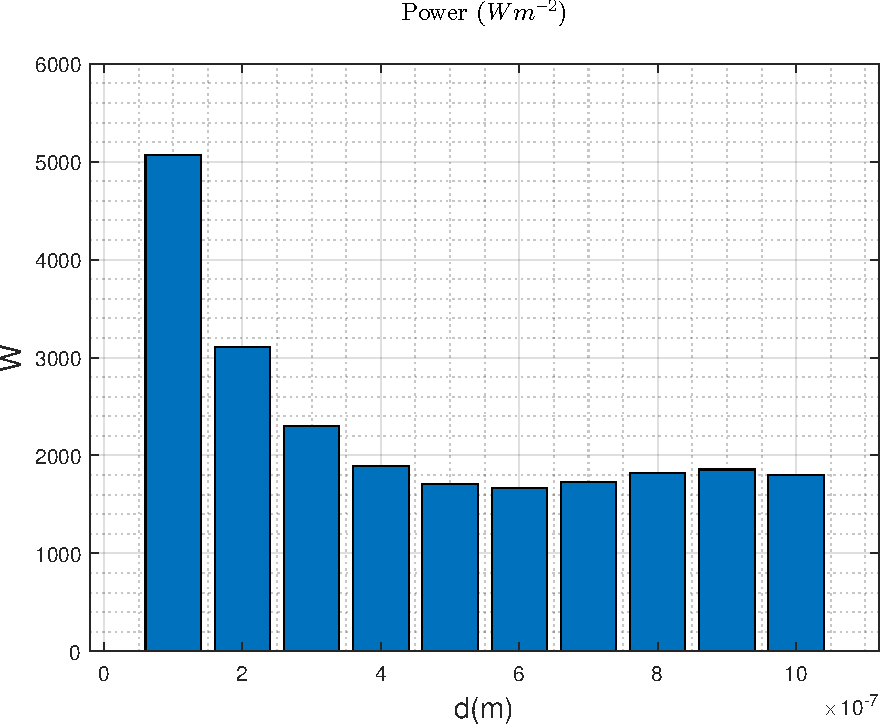
\includegraphics[width=0.65\textwidth]{figuras/Resultados/radiacion/p_Eg_SiSi.pdf}
	\caption{Potencia por unidad de área de la radiación por campo cercano en el rango de longitudes de onda de energía mayor e igual a 0.7eV.}
	\label{fig:p_Eg_SiSi}
\end{figure}
Como se puede observar en la figura \ref{fig:p_Eg_SiSi} al aumentar el rango de integración o disminuir la banda energética, aumenta la potencia que llega por radiación, lo que produce el aumento de energía que se puede convertir en electricidad.
%% RELACION ENTRE COND Y RAD
\subsection{Relación de transmisión por conducción y radiación}
Para tener una primera mejor idea de los valores numéricos de los resultados obtenidos de las simulaciones de transmisión de calor por conducción y radiación de campo cercano se recolectan en la tabla \ref{tab:condTerSiSiO2Si}, estando en notación científica y con los decimales necesarios para una clara diferenciación de los resultados con el cambio de la distancia de separación entre emisor y célula.
\begin{table}[H]
	\centering
		\begin{tabular}{|c||c|c|c|c||c|c|}
		\hline
			\multirow{2}{*}{ }& \multicolumn{6}{c|}{\textbf{\large Potencias según como se transmite el calor}}\\ \cline{2-7}
		  & \multicolumn{4}{c||}{Conducción (W/nº nano-espaciadores)}& \multicolumn{2}{c|}{Radiación $(W/m^2)$}\\ \hline
			Dist. (nm)&$P_{Normal}$&$P_{R_c-Empirico}$&$P_{Porosidad25}$&$P_{Porosidad50}$&$P_{Eg>0.7eV}$&$P_{full}$\\ \hline \hline
			100&6,31E-02&1,69E-03&4,67E-02&2,30E-02&5,07E+03&1,65E+05\\ \hline
			200&3,99E-02&1,66E-03&2,78E-02&1,26E-02&3,11E+03&1,10E+05\\ \hline
			300&2,93E-02&1,63E-03&1,99E-02&8,69E-03&2,30E+03&8,51E+04\\ \hline
			400&2,32E-02&1,60E-03&1,55E-02&6,63E-03&1,90E+03&7,01E+04\\ \hline
			500&1,92E-02&1,58E-03&1,27E-02&5,36E-03&1,70E+03&6,02E+04\\ \hline
			600&1,64E-02&1,55E-03&1,08E-02&4,50E-03&1,66E+03&5,32E+04\\ \hline
			700&1,43E-02&1,53E-03&9,33E-03&3,88E-03&1,72E+03&4,80E+04\\ \hline
			800&1,27E-02&1,50E-03&8,24E-03&3,41E-03&1,82E+03&4,43E+04\\ \hline
			900&1,14E-02&1,48E-03&7,38E-03&3,04E-03&1,86E+03&4,14E+04\\ \hline
			1000&1,04E-02&1,46E-03&6,68E-03&2,74E-03&1,80E+03&3,93E+04\\ \hline
		\end{tabular}
	\caption{Tabla de resultados de las simulaciones de conducción y radiación de campo cercano para diferentes alturas del nano-espaciador. Flujos de calor del TPV $Si-SiO_2-Si$ para diferentes alturas del nano-espaciador, para los casos sin $R_c$ y con $R_c$ igual a $4 \cdot 10^{-6} \ m^2 K/W$ \cite{nf_TPV_Pillars_SiO2}, y sin $R_c$ pero con las proporciones de las porosidades de \cite{ThermalConductivity_SiO2_2018} para un 25\% y un 50\%.}
	\label{tab:condTerSiSiO2Si}
\end{table}
\begin{figure}[H]
	\centering
	%% Si-SiO2-Si Eg
	\begin{subfigure}[b]{0.49\textwidth}
		\centering
		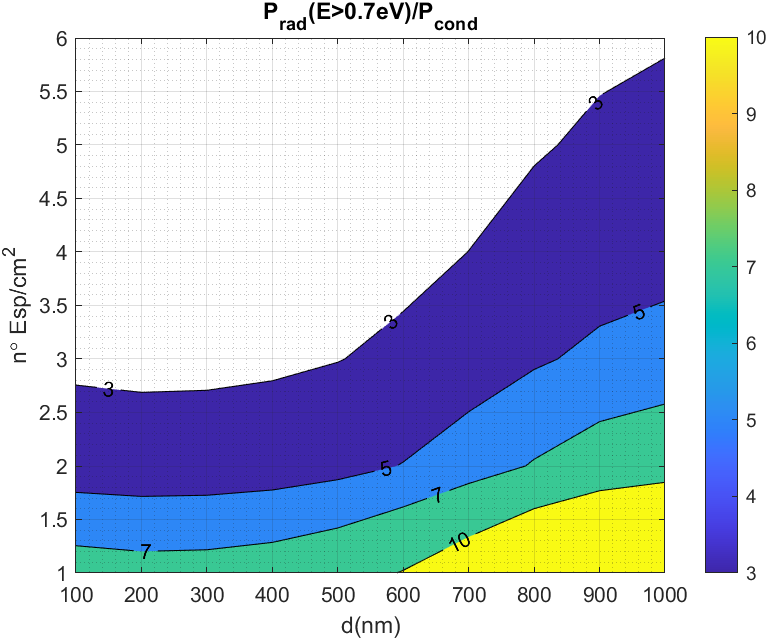
\includegraphics[width=1.00\textwidth]{figuras/Resultados/RelacionCondRad/SiSi.png}
		\caption{Relación para Eg$>$0.7 eV}
		\label{fig:rel_SiSiO2Si}
	\end{subfigure}
	\hfill
	\begin{subfigure}[b]{0.49\textwidth}
		\centering
		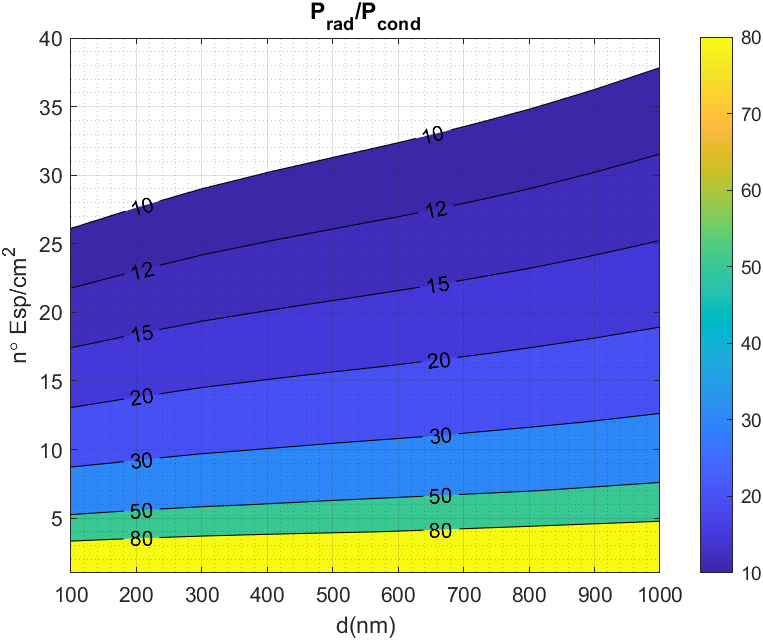
\includegraphics[width=1.00\textwidth]{figuras/Resultados/RelacionCondRad/SiSi_full.png}
		\caption{Relación en todo el rango disponible}
		\label{fig:rel_SiSiO2Si_full}
	\end{subfigure}
	\hfill
	\begin{subfigure}[b]{0.49\textwidth}
		\centering
		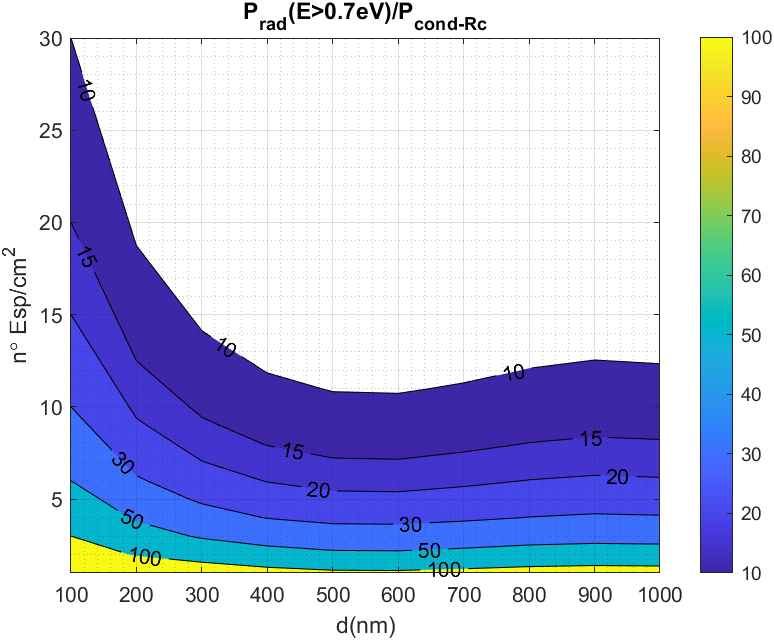
\includegraphics[width=1.00\textwidth]{figuras/Resultados/RelacionCondRad/SiSi_Rc.png}
		\caption{Relación para Eg$>$0.7 eV y con $R_c$}
		\label{fig:rel_SiSiO2Si_Rc}
	\end{subfigure}
	\hfill
	\begin{subfigure}[b]{0.49\textwidth}
		\centering
		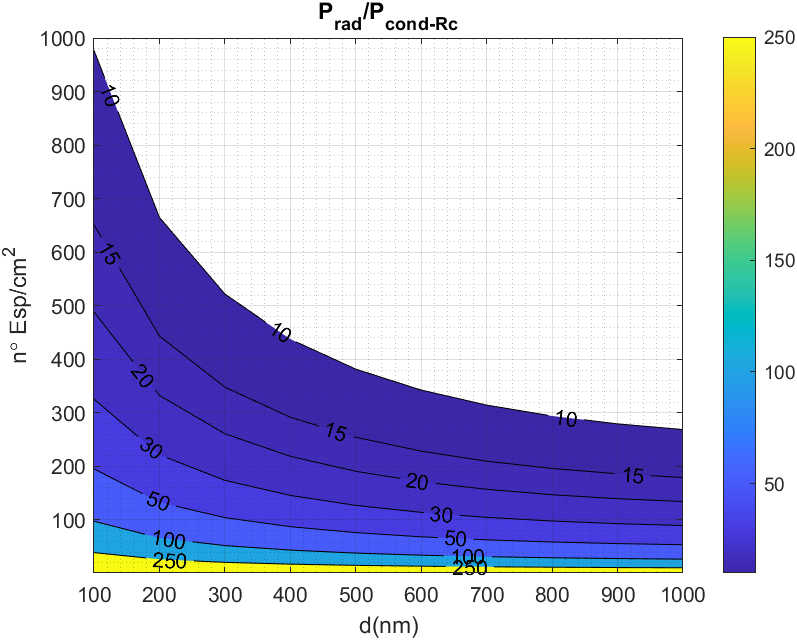
\includegraphics[width=1.00\textwidth]{figuras/Resultados/RelacionCondRad/SiSi_Rc_full_10.png}
		\caption{Relación en todo el rango disponible y con $R_c$}
		\label{fig:rel_SiSiO2Si_Rc_full}
	\end{subfigure}
	\caption{Relación de la potencia radiada en un 1 $cm^2$ y conducción por cantidad de espaciadores en el centímetro cuadrado para el rango de Eg$>$ 0.7 eV sin $r_c$ (\subref{fig:rel_SiSiO2Si}) y con $R_c$ (\subref{fig:rel_SiSiO2Si_Rc}), y en todo el rango disponible de longitudes de onda sin (\subref{fig:rel_SiSiO2Si_full}) y con $R_c$ (\subref{fig:rel_SiSiO2Si_Rc_full}).}
	\label{fig:relation_SiSiO2Si}
\end{figure}
La cantidad de nano-espaciadores necesarios para varias relaciones entre la potencia conducida con y sin $R_c$ y la potencia radiada por campo cercano  se representan en las figuras \ref{fig:relation_SiSiO2Si}. Se observa como el efecto de la resistencia de contacto aumenta favorablemente el número de espaciadores necesarios para relaciones mayores de 10 y se observa como al aumentar la cantidad de radiación que se utiliza en la célula, aumenta el número de espaciadores que se pueden colocar para separar ambas placas, lo que implica que se puede mantener más estable la distancia de separación entre el emisor y la célula.\\\\
 Para los casos con $R_c$ se pasa de unos 30 nano-espaciadores a unos 1000 nano-espaciadores máximos y como mínimo se pasa de unos $\sim$10 a más de 250 nano-espaciadores para una relación de 10.
%%% AHORA EL CASO DE Si SiO2 y Ge
\section{Resultados de las simulaciones para una TPV de Si-SiO2-Ge}
Ahora se procede a estudiar un caso más realista del sistema TPV con una célula de $Ge$ cuya banda energética es de 0.7 eV. Cuyos resultados de conducción son muy parecidos al caso de célula de $Si$ , siendo su relación de potencia (figura \ref{fig:relPrc_SiSiO2Ge}) un poco mayor.
\begin{figure}[H]
	\centering
	%% Si-SiO2-Si Eg
	\begin{subfigure}[b]{0.49\textwidth}
		\centering
		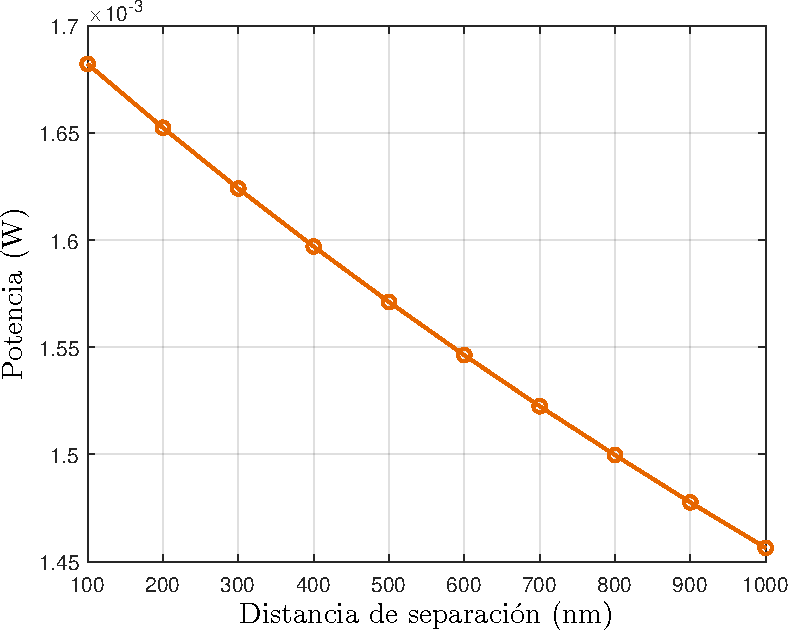
\includegraphics[width=1.00\textwidth]{figuras/Resultados/conduccion/pdf/Prc2_SiSiO2Ge.pdf}
		\caption{Potencias de conducción}
		\label{fig:Prc_SiSiO2Ge}
	\end{subfigure}
	\hfill
	\begin{subfigure}[b]{0.49\textwidth}
		\centering
		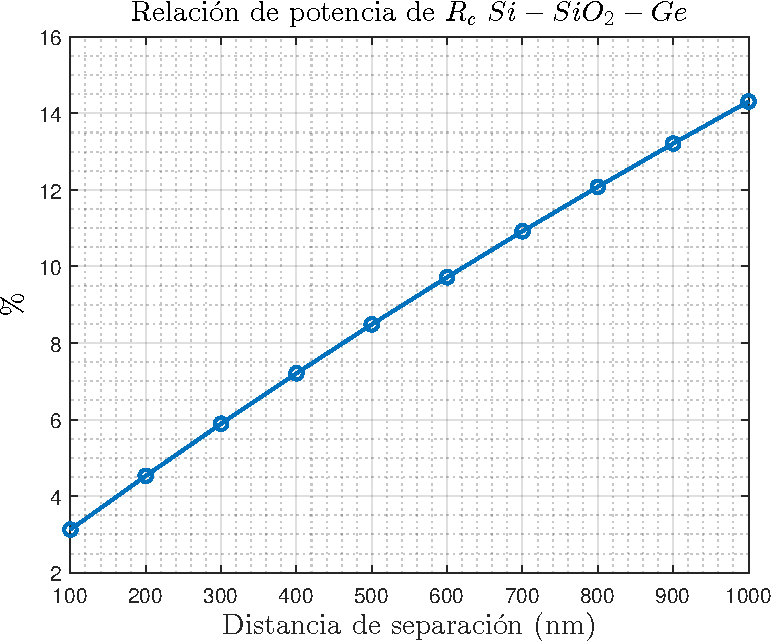
\includegraphics[width=0.92\textwidth]{figuras/Resultados/conduccion/pdf/relPrc_SiSiO2Ge.pdf}
		\caption{Relación de $P_{R_c}$ respecto a $P$}
		\label{fig:relPrc_SiSiO2Ge}
	\end{subfigure}
	\caption{(\subref{fig:Prc_SiSiO2Ge}) Potencia de conducción con y si resistencia de contacto empírica \cite{nf_TPV_Pillars_SiO2}. (\subref{fig:relPrc_SiSiO2Ge}) Relación de la potencia de conducción del caso con resistencia de contacto respecto a la potencia de conducción sin resistencia de contacto.}
	\label{fig:Pcond_SiSiO2Ge}
\end{figure}
De las simulaciones de radiación de campo cercano se obtienen también resultados muy parecidos a los obtenidos en el caso de la célula de $Si$ (figura \ref{fig:SiSi_vs_SiGe}), solo mostrándose hasta los $\sim$14$\mu m$ de longitud de onda, donde se observa como al disminuir la distancia de separación aumenta la potencia de radiación monocromática (figura \ref{fig:rad_SiGe}).
\begin{figure}[H]
\centering
\begin{subfigure}[b]{0.49\textwidth}
	\centering
		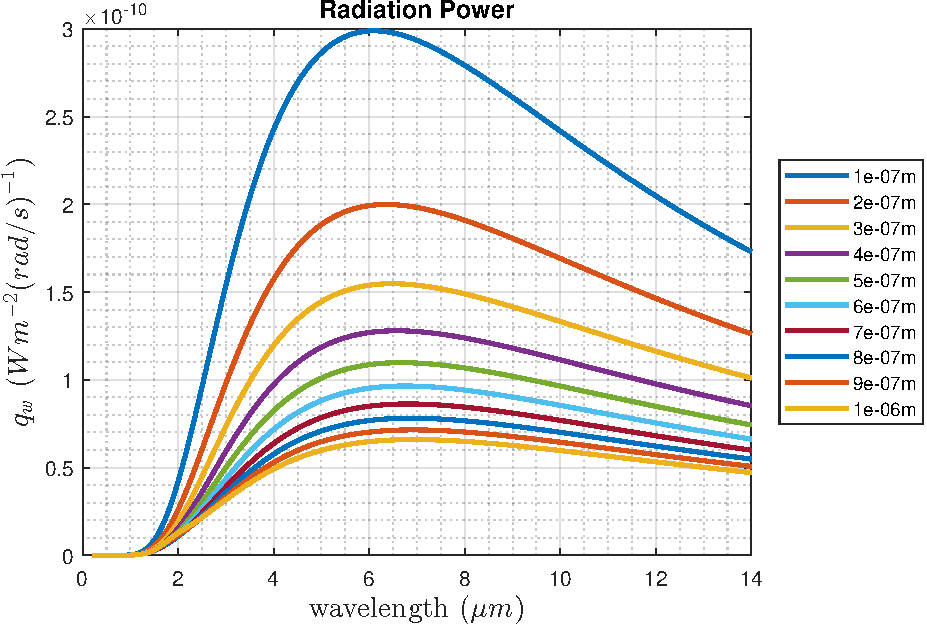
\includegraphics[width=1.00\textwidth]{figuras/Resultados/radiacion/SiGe.pdf}
	\caption{Potencia monocromática para varias $d$}
	\label{fig:rad_SiGe}
\end{subfigure}
\hfill
\begin{subfigure}[b]{0.49\textwidth}
	\centering
		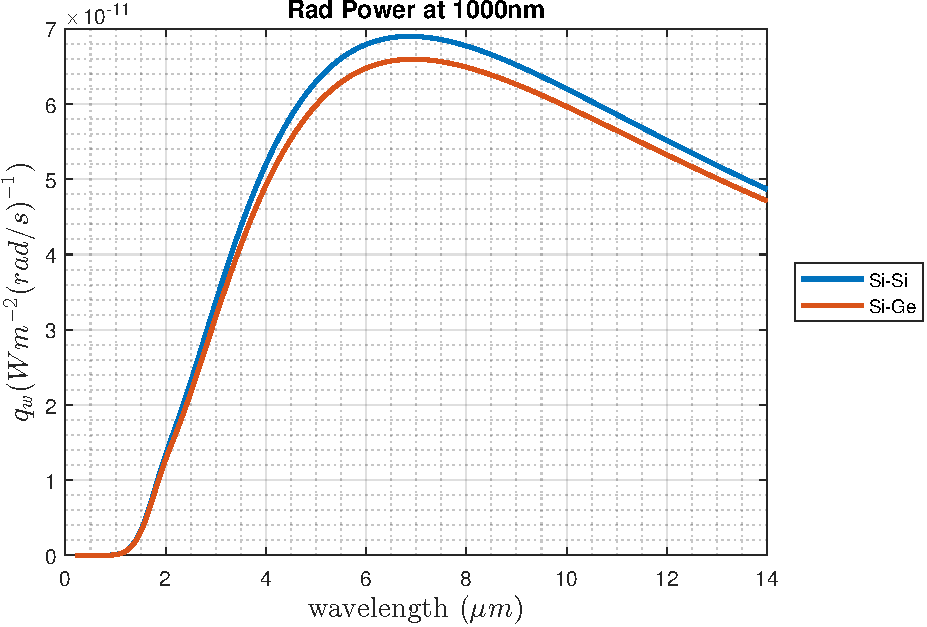
\includegraphics[width=1.00\textwidth]{figuras/Resultados/radiacion/SiSi_vs_SiGe.pdf}
	\caption{Comparación de células de $Si$ y $Ge$}
	\label{fig:SiSi_vs_SiGe}
\end{subfigure}
\caption{(\subref{fig:rad_SiGe}) Potencia radiada por campo cercano para diferentes separación entre placas para un emisor de $Si$ a 800\textdegree C y una célula de $Ge$ a 25\textdegree C. (\subref{fig:SiSi_vs_SiGe}) Comparación de la potencia radiada monocromática para una separación de 1000nm entre el sistema $Si-Si$ y $Si-Ge$.}
\label{fig:rads_SiGe}
\end{figure}
Para la obtención de las potencias de radiación se procede a realizar la integral en el rango de longitudes de onda cuya energía es mayor a los 0.7 eV, obteniéndose potencias alrededor de los $10^3 \ W/m^2$ (figura \ref{fig:p_Eg_SiGe}). Para todo el rango disponible de longitudes de onda se obtiene alrededor de los $10^4 \ W/m^2$ con un máximo de $\sim$1.5$10^5 \ W/m^2$ (figura \ref{fig:p_full_SiGe} y tabla ref{tab:SiSiO2Ge}). 
\begin{figure}[H]
\centering
\begin{subfigure}[b]{0.49\textwidth}
	\centering
		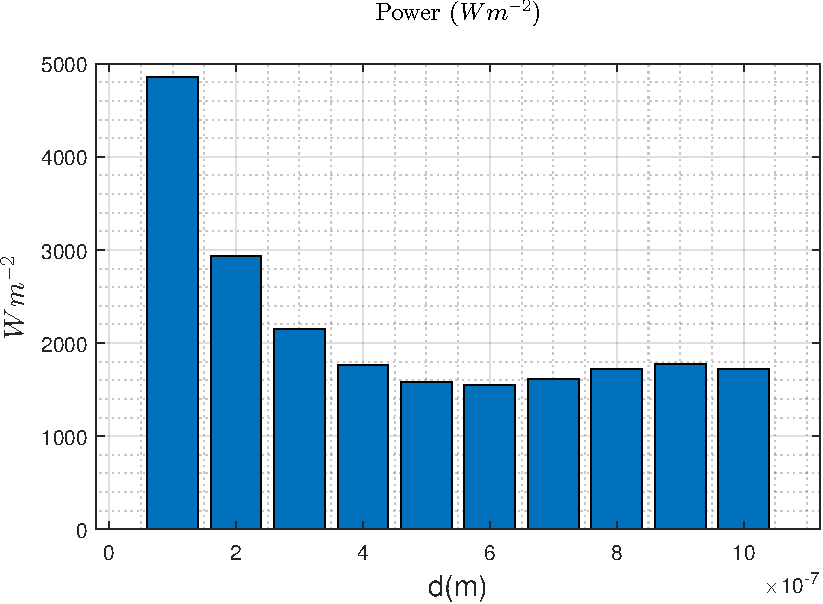
\includegraphics[width=1.00\textwidth]{figuras/Resultados/radiacion/p_Eg_SiGe.pdf}
	\caption{Potencia para Eg$>$0.7eV}
	\label{fig:p_Eg_SiGe}
\end{subfigure}
\begin{subfigure}[b]{0.49\textwidth}
	\centering
		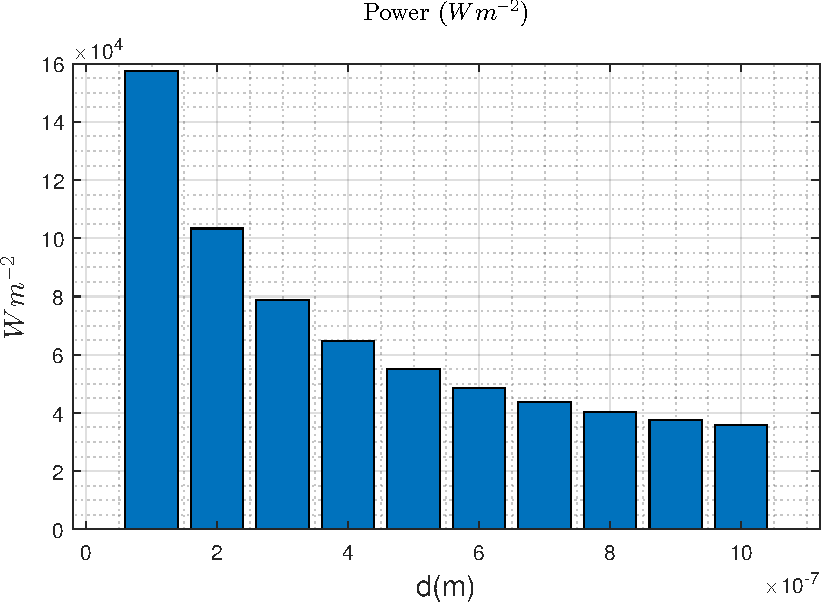
\includegraphics[width=1.00\textwidth]{figuras/Resultados/radiacion/p_full_SiGe.pdf}
	\caption{Potencia hasta $\sim$14$\mu m$}
	\label{fig:p_full_SiGe}
\end{subfigure}
	\caption[Potencias por unidad de área para la radiación de campo cercano para el sistema $Si-SiO_2-Ge$ para diferentes alturas del nano-espaciador]{Potencias por unidad de área para la radiación de campo cercano para el sistema $Si-SiO_2-Ge$ para diferentes alturas del nano-espaciador. (\subref{fig:p_Eg_SiGe}) Potencias en el rango de todas las longitudes de onda de energía mayor a 0.7 eV. (\subref{fig:p_full_SiGe}) Potencias en todo el rango disponible de longitudes de onda, hasta las $\sim$14$\mu m$.}
	\label{fig:p_SiGe}
\end{figure}
Para facilitar la revisión de los resultados obtenidos de las simulaciones se agrupan en la tabla \ref{tab:SiSiO2Ge}, donde se presentan en notación científica para facilitar la observación de la magnitud de los resultados.
\begin{table}[H]
	\centering
		\begin{tabular}{|c||c|c||c|c|}
		\hline
\multirow{2}{*}{ }& \multicolumn{4}{c|}{\textbf{\large Potencias según transmisión del calor}}\\ \cline{2-5}
& \multicolumn{2}{c||}{Conducción (W/nº esp.)}& \multicolumn{2}{c|}{Radiación $(W/m^2)$}\\ \hline
Dist. (nm)&$P_{Normal}$&$P_{R_c-Empirico}$&$P_{Eg>0.7eV}$&$P_{full}$\\ \hline \hline
100&5,38E-02&1,68E-03&4,87E+03&1,54E+05\\ \hline 
200&3,65E-02&1,65E-03&2,94E+03&1,01E+05\\ \hline 
300&2,76E-02&1,62E-03&2,16E+03&7,71E+04\\ \hline 
400&2,22E-02&1,60E-03&1,77E+03&6,31E+04\\ \hline 
500&1,85E-02&1,57E-03&1,59E+03&5,38E+04\\ \hline 
600&1,59E-02&1,55E-03&1,55E+03&4,74E+04\\ \hline 
700&1,39E-02&1,52E-03&1,62E+03&4,27E+04\\ \hline 
800&1,24E-02&1,50E-03&1,73E+03&3,93E+04\\ \hline 
900&1,12E-02&1,48E-03&1,78E+03&3,67E+04\\ \hline 
1000&1,02E-02&1,46E-03&1,73E+03&3,49E+04\\ \hline 
		\end{tabular}
	\caption{Tabla de las potencias de resultado de las simulaciones de transmisión de calor por radiación de campo cercano y conducción para el sistema TPV $Si-SiO_2-Ge$.}
	\label{tab:SiSiO2Ge}
\end{table}
Hay que tener en cuenta que para un centímetro cuadrado las columnas de la transmisión de calor por radiación de la tabla \ref{tab:SiSiO2Ge} se ven multiplicadas por $10^{-4}$, por lo tanto, la potencia de radiación con $E_g>0.7eV$ en un centímetro cuadrado es solamente $\sim$10 mayor que la potencia conducida sin resistencia de contacto para un nano-espaciador, pero $\sim$100 veces mayor que la potencia conducida con resistencia de contacto.
\begin{figure}[H]
	\centering
	%% Si-SiO2-Si Eg
	\begin{subfigure}[b]{0.49\textwidth}
		\centering
		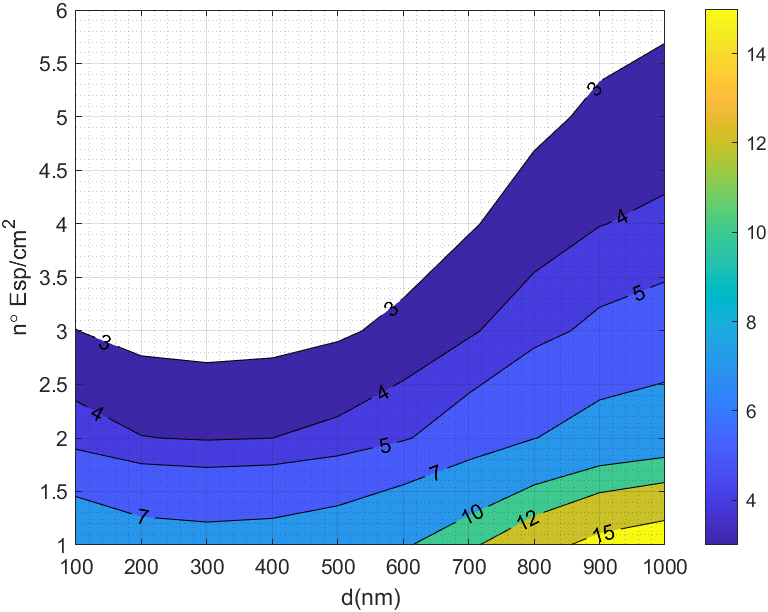
\includegraphics[width=1.00\textwidth]{figuras/Resultados/RelacionCondRad/SiGe.png}
		\caption{$E>0.7eV$}
		\label{fig:rel_SiSiO2Ge}
	\end{subfigure}
	\hfill
	\begin{subfigure}[b]{0.49\textwidth}
		\centering
		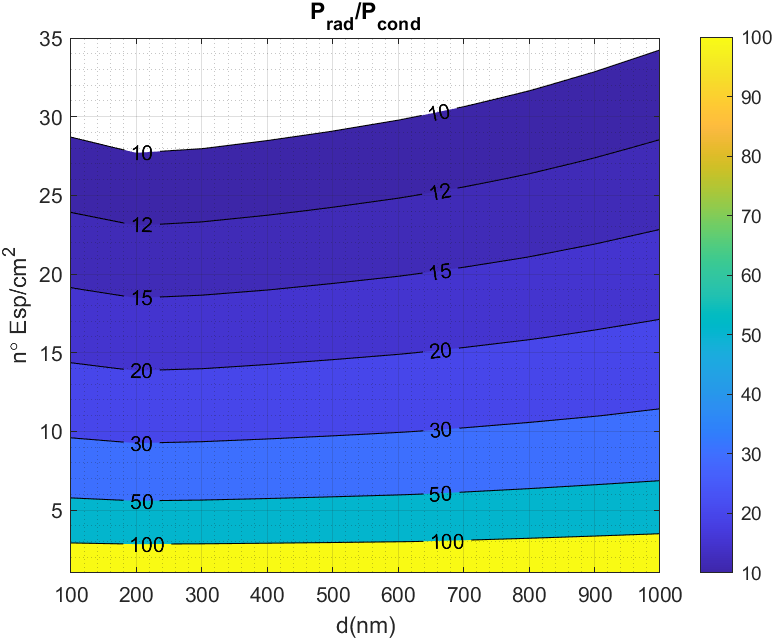
\includegraphics[width=1.00\textwidth]{figuras/Resultados/RelacionCondRad/SiGe_full.png}
		\caption{rango completo}
		\label{fig:rel_SiSiO2Ge_full}
	\end{subfigure}
	\hfill
	\begin{subfigure}[b]{0.49\textwidth}
		\centering
		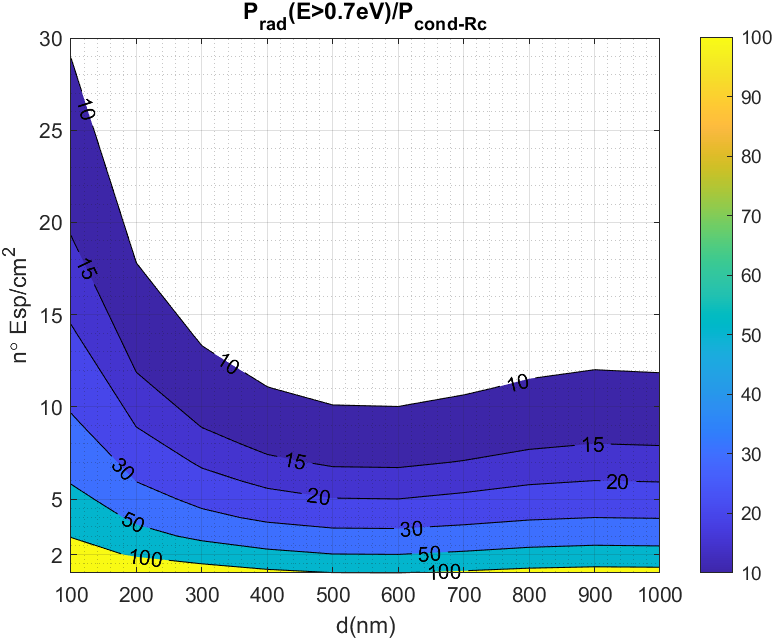
\includegraphics[width=1.00\textwidth]{figuras/Resultados/RelacionCondRad/SiGe_Rc.png}
		\caption{$E>0.7eV$ y con $R_c$}
		\label{fig:rel_SiSiO2Ge_Rc}
	\end{subfigure}
	\hfill
	\begin{subfigure}[b]{0.49\textwidth}
		\centering
		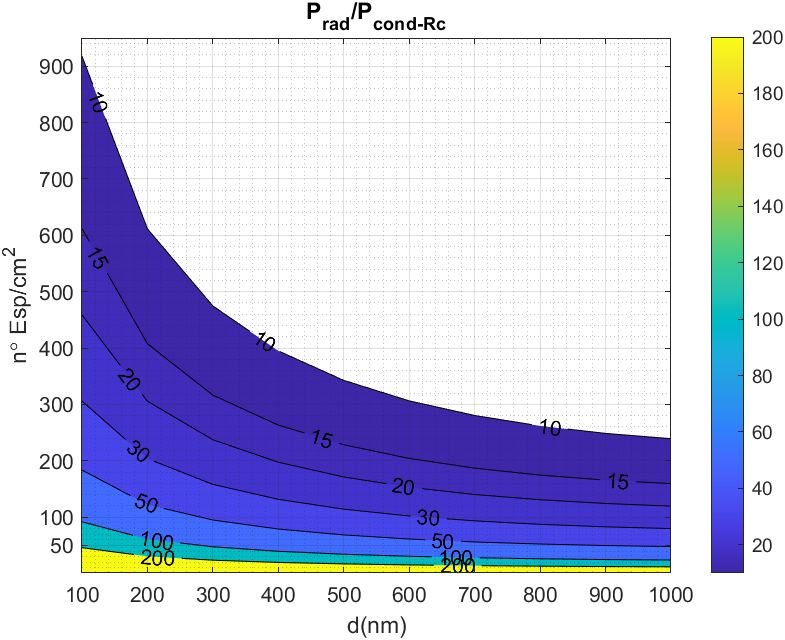
\includegraphics[width=1.00\textwidth]{figuras/Resultados/RelacionCondRad/SiGe_Rc_full_10.png}
		\caption{rango completo y con $R_c$}
		\label{fig:rel_SiSiO2Ge_Rc_full}
	\end{subfigure}
	\caption[Relaciones entre la potencia de conducción para diferentes cantidades de nano-espaciadores y la potencia de radiación en 1$cm^2$ para diferentes distancias de separación o alturas de nano-espaciador]{Relaciones entre la potencia de conducción para diferentes cantidades de nano-espaciadores y la potencia de radiación en 1$cm^2$ para diferentes distancias de separación o alturas de nano-espaciador. (\subref{fig:rel_SiSiO2Ge}) Relación de las potencias sin resistencia de contacto y la radiación en un rango de energía mayor a 0.7eV. (\subref{fig:rel_SiSiO2Ge_full}) Relación de las potencias sin resistencia de contacto y la radiación en todo el rango disponible. (\subref{fig:rel_SiSiO2Ge_Rc}) Relación de las potencias con resistencia de contacto \cite{nf_TPV_Pillars_SiO2} y la radiación en un rango de energía mayor a 0.7eV. (\subref{fig:rel_SiSiO2Ge_Rc_full}) Relación de las potencias con resistencia de contacto \cite{nf_TPV_Pillars_SiO2} y la radiación en todo el rango disponible.}
	\label{fig:relation_SiSiO2Ge}
\end{figure}
Como se observa en las figuras \ref{fig:relation_SiSiO2Ge} la resistencia de contacto tiene un efecto muy favorable sobre el sistema TPV aumentando la relación entre las potencias y el número de espaciadores que se pueden utilizar para separar el emisor y la célula. También afecta a la forma de la curva de relaciones, cambiando el sentido del incremento de los números de espaciadores a una relación de 10 por cada distancia de separación porque cuando no existe resistencia de contacto la resistencia del nano-espaciador depende principalmente de su altura (figuras \ref{fig:rel_SiSiO2Ge} y \ref{fig:rel_SiSiO2Ge_full}) y cuando existe resistencia de contacto el flujo de calor por conducción es tan pequeño respecto al de radiación que se puede considerar casi una recta y depende principalmente de la radiación por campo cercano (figuras \ref{fig:rel_SiSiO2Ge_Rc} y \ref{fig:rel_SiSiO2Ge_Rc_full}). \\\\
\section{Resultados de las simulaciones para una TPV de SS-SiO2-Ge}
Un caso importante a estudiar es cuando el emisor es de acero inoxidable ($SS$) para la recuperación de calor residual porque en la industria se utiliza mucho el acero inoxidable como material para calderas, tuberías, entre otros componentes o máquinas que alcanzan altas temperaturas y que tienen que se enfriadas mediante un intercambiadores de calor que se conectan a turbinas de vapor para recuperar parte de la energía, presentando el problema de trabajar con fluidos y partes móviles que necesitan mantenimiento.\\\\
Para las simulaciones de transmisión de calor por conducción se estudian los efectos de resistencias de contacto aún mayores, obtenidas las conductancias de contacto entre dos trozos de acero 304 y mediante las ecuaciones \eqref{eq:relacion_conductividadesTermicas} y \eqref{eq:relacion_Rc} se obtienen las resistencia de contacto para una presión de $\sim$1 GPa por ser un valor con menor error respecto al modelo matemático \cite{experimental_Rc_SS}, siendo dicho valor aproximadamente unos 1000 $W/(m^2 K)$ .\\\\
La nueva resistencia de contacto calculada es $5.5\cdot 10^{-3} \ m^2 K/W$ y se toma un valor intermedio entre dicha resistencia de contacto y la resistencia de contacto empírica de $4\cdot 10^{-6} \ m^2 K/W$ \cite{nf_TPV_Pillars_SiO2} para obtener en mayor detalle los efectos de la resistencia de contacto sobre el flujo de calor por conducción, siendo el valor de dicha resistencia de contacto calculada intermedia unos $\sim 2.75\cdot 10^{-3} \ m^2 K/W$.
\begin{figure}[H]
	\centering
	\begin{subfigure}[b]{0.49\textwidth}
		\centering
			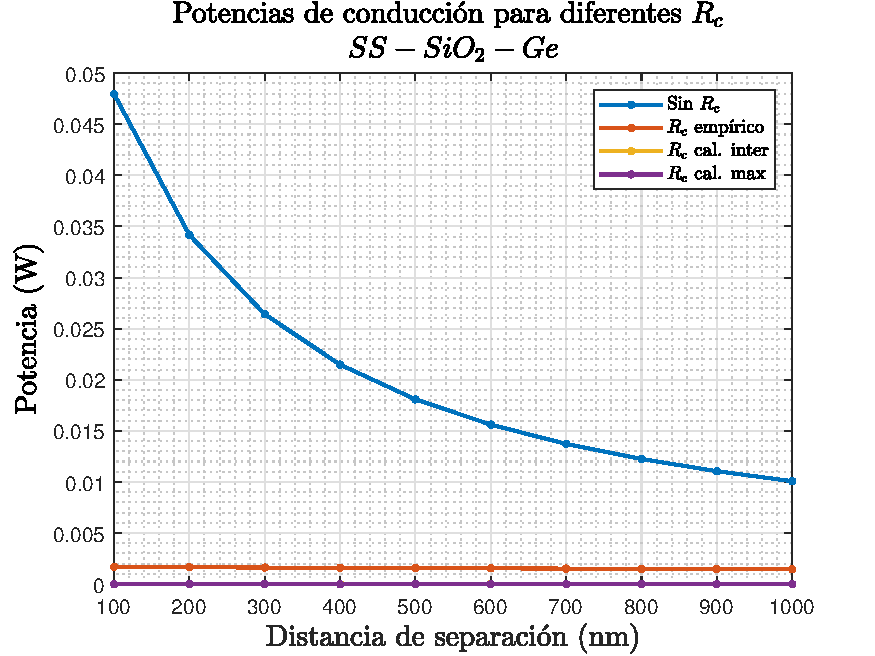
\includegraphics[width=1.00\textwidth]{figuras/Resultados/conduccion/pdf/Prcs_SsSiO2Ge.pdf}
		\caption{Potencias de conducción}
		\label{fig:Prcs_SsSiO2Ge}
	\end{subfigure}
	\hfill
	\begin{subfigure}[b]{0.49\textwidth}
		\centering
			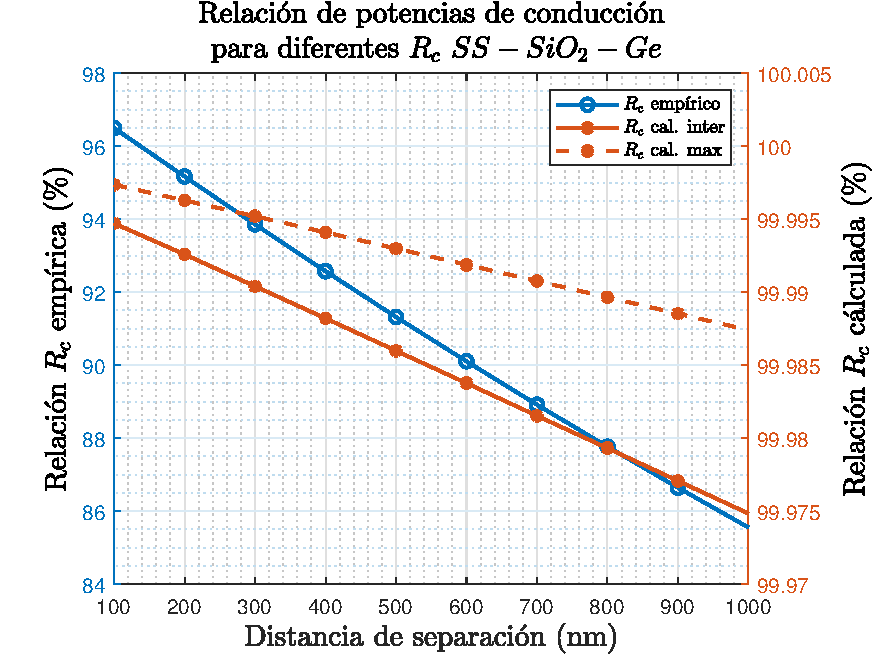
\includegraphics[width=1.00\textwidth]{figuras/Resultados/conduccion/pdf/relPrcs_SsSiO2Ge.pdf}
		\caption{Relaciones de potencias con $R_c$ respecto sin $R_c$}
		\label{fig:relPrcs_SsSiO2Ge}
	\end{subfigure}
	\caption{ (\subref{fig:Prcs_SsSiO2Ge}) Potencias de conducción sin y con resistencias de contacto para un emisor de $SS$, las resistencias de contacto son de $4\cdot 10^{-6} \ m^2 K/W$ para la $R_c$ empírica, $5.5\cdot 10^{-3} \ m^2 K/W$ para la $R_c$ cal. max y $2.75\cdot 10^{-3} \ m^2 K/W$ para la $R_c$ cal. inter. (\subref{fig:relPrcs_SsSiO2Ge}) Relaciones de las potencias con $R_c$ respecto a la potencia conducida sin $R_c$.}
	\label{fig:Pcond_SsSiO2Ge}
\end{figure}
Al aumentar la resistencia de contacto disminuye el flujo de calor por conducción porque aumenta la resistencia térmica total como se puede observar e la figura \ref{fig:Prcs_SsSiO2Ge} donde las resistencia de contacto calculadas son tan pequeñas que casi no se ven. Para tener una mejor visualización de los efectos de las resistencias de contacto se calcula la relación de cada una respecto a la potencia conducida sin resistencia de contacto, obteniéndose a como es de esperar que para las resistencias de contacto calculadas, es decir, las de mayor valor, la relación es muy pequeña menos de un 0.03\%, a diferencia de la $R_c$ empírica que comparada con las relaciones de los casos de TPV $Si-SiO_2-Ge$ es un poco mayor, superando el 3\% como mínimo y aproximadamente uno 14.5\% en su máximo.\\\\
Dada la alta complejidad de la variación de la resistencia de contacto no se obtiene un modelo matemático que relaciona la potencia de conducción por resistencia de contacto y por altura de nano-espaciador.\\\\
Para la simulación de radiación de campo cercano solo se considera los resultados en el rango de energía mayor a 0.7eV o $\sim$1.8 $\mu m$ porque los datos de el índice de refracción $n$ y índice de extinción $k$ llegan hasta los 1.2 $\mu m$ \cite{ss_optical_2017}, realizando una extrapolación lineal hasta los 1.8$\mu m$ para poder obtener las potencias de radiación para diferentes distancias de separación.
\begin{figure}[H]
	\centering
	\begin{subfigure}[b]{0.49\textwidth}
	\centering
		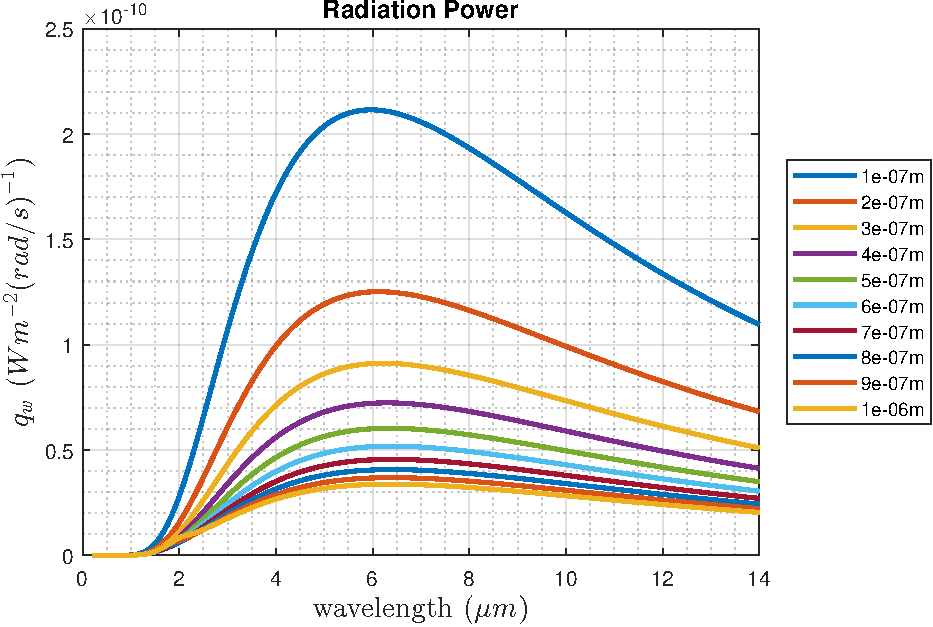
\includegraphics[width=1.00\textwidth]{figuras/Resultados/radiacion/SsGe.pdf}
	\caption{Potencia monocromática}
	\label{fig:SsGe}
\end{subfigure}
\begin{subfigure}[b]{0.49\textwidth}
	\centering
		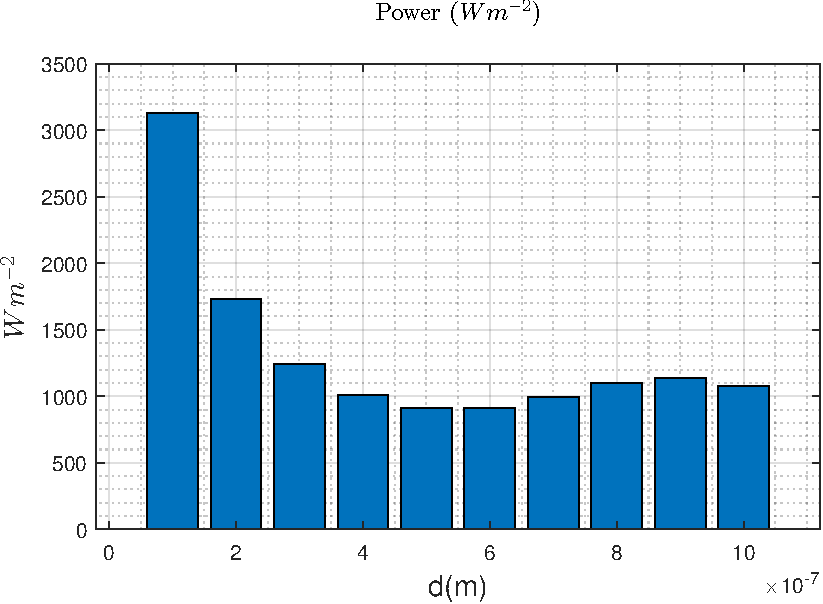
\includegraphics[width=1.00\textwidth]{figuras/Resultados/radiacion/p_Eg_SsGe.pdf}
	\caption{Potencia hasta 0.7 eV}
	\label{fig:p_Eg_SsGe}
\end{subfigure}
\caption{(\subref{fig:SsGe}) Potencia radiada monocromática por campo cercano para un emisor de $SS$ y una célula de $Ge$. (\subref{fig:p_Eg_SsGe}) Potencia radiada para un rango de longitudes de onda cuya energía es mayor a los 0.7eV ($\sim 1.8 \ \mu m$).}
	\label{fig:rad_SsGe}
\end{figure}
Las potencias por unidad de área se encuentran en general en el rango de los miles de $W/m^2$, siendo inferior a la del $Si$ pero no por un factor de magnitud.
\begin{table}[H]
	\centering
		\begin{tabular}{|c||c|c|c|c||c|}
		\hline
		\multirow{2}{*}{ }& \multicolumn{5}{c|}{\textbf{\large Potencias según transmisión del calor}}\\ \cline{2-6}
& \multicolumn{4}{c||}{Conducción (W/nº esp.)}& Radiación $(W/m^2)$\\ \hline
Dist. (nm)&$P_{Normal}$&$P_{R_c-Cal.Max}$&$P_{R_c-Cal.Inter}$&$P_{R_c-Empirico}$&$P_{Eg>0.7eV}$\\ \hline \hline
100&4,80E-02&1,26815E-06&2,53438E-06&1,68E-03&3,13E+03\\ \hline 
200&3,42E-02&1,26813E-06&2,53431E-06&1,65E-03&1,73E+03\\ \hline 
300&2,64E-02&1,26811E-06&2,53424E-06&1,62E-03&1,24E+03\\ \hline 
400&2,15E-02&1,26809E-06&2,53417E-06&1,60E-03&1,01E+03\\ \hline 
500&1,81E-02&1,26808E-06&2,53410E-06&1,57E-03&9,11E+02\\ \hline 
600&1,56E-02&1,26806E-06&2,53403E-06&1,54E-03&9,10E+02\\ \hline 
700&1,37E-02&1,26804E-06&2,53396E-06&1,52E-03&9,93E+02\\ \hline 
800&1,22E-02&1,26802E-06&2,53388E-06&1,50E-03&1,10E+03\\ \hline 
900&1,11E-02&1,26800E-06&2,53381E-06&1,48E-03&1,14E+03\\ \hline 
1000&1,01E-02&1,26799E-06&2,53374E-06&1,45E-03&1,08E+03\\ \hline 
		\end{tabular}
	\caption{Tabla de recopilación de los resultados de las simulaciones de transmisión de calor por conducción y radiación de campo cercano para una TPV de emisor de $SS$.}
	\label{tab:SsSiO2Ge}
\end{table}
 Se recopilan los resultados de las simulaciones en la tabla \ref{tab:SsSiO2Ge} y se observa que para un centímetro cuadrado de superficie de radiación las potencias se encuentran en el rango de los 0.1 $W$, no siendo suficientemente mayor para que para un nano-espaciador la relación de las potencias para todas las distancias sea $\sim$10 (figura \ref{fig:rel_SsSiO2Ge}), pero para los casos con resistencia de contacto sí que se cumple. 
\begin{figure}[H]
	\centering
	\begin{subfigure}[b]{0.49\textwidth}
		\centering
			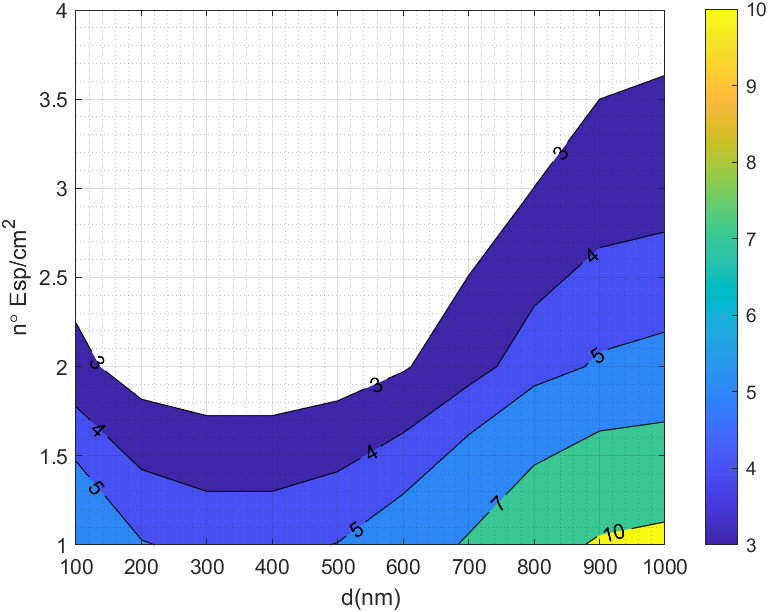
\includegraphics[width=1.00\textwidth]{figuras/Resultados/RelacionCondRad/SS.png}
		\caption{Sin $R_c$}
		\label{fig:rel_SsSiO2Ge}
	\end{subfigure}
	\hfill
	\begin{subfigure}[b]{0.49\textwidth}
		\centering
			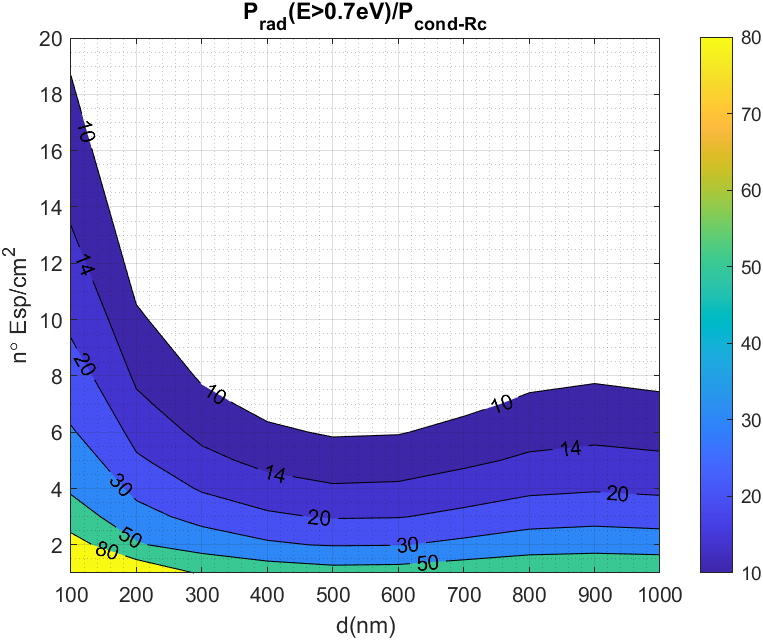
\includegraphics[width=1.00\textwidth]{figuras/Resultados/RelacionCondRad/SS_Rc_empirico.png}
		\caption{$R_c$ empírica}
		\label{fig:rel_SsSiO2Ge_Rc_emp}
	\end{subfigure}
	\hfill
	\begin{subfigure}[b]{0.49\textwidth}
		\centering
			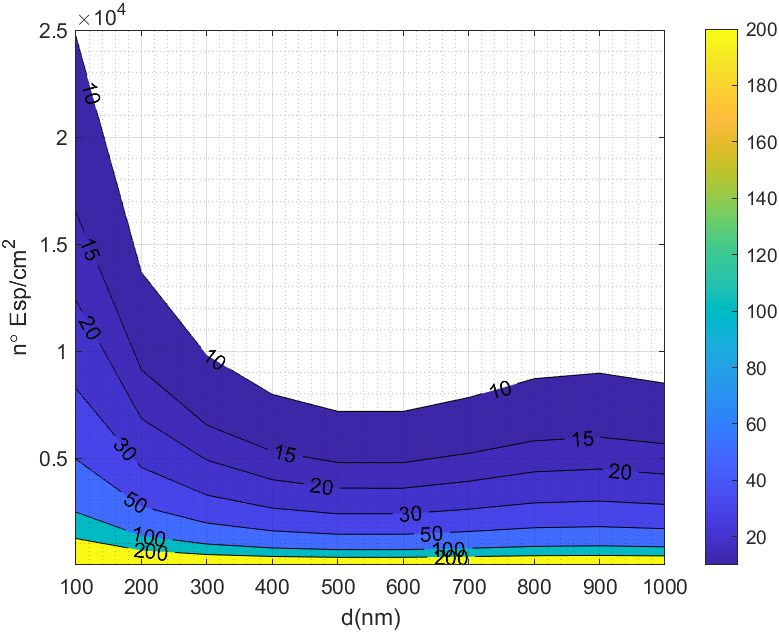
\includegraphics[width=1.00\textwidth]{figuras/Resultados/RelacionCondRad/SS_Rc.png}
		\caption{$R_c$ calculada máxima}
		\label{fig:rel_SsSiO2Ge_Rc_max}
	\end{subfigure}
	\hfill
	\begin{subfigure}[b]{0.49\textwidth}
		\centering
			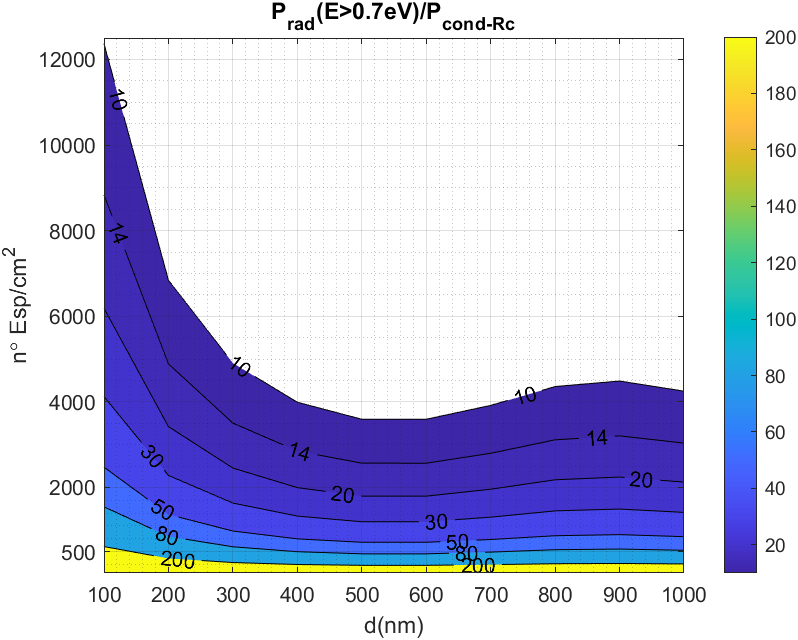
\includegraphics[width=1.00\textwidth]{figuras/Resultados/RelacionCondRad/SS_Rc_Intermedio.png}
		\caption{$R_c$ calculada intermedia}
		\label{fig:rel_SsSiO2Ge_Rc_inter}
	\end{subfigure}
	\caption[Relación de las potencias de conducción y radiación para un emisor de $SS$ según el número de nano-espaciadores y la altura de los nano-espaciadores para un emisor y célula de 1 $cm^2$]{Relación de las potencias de conducción y radiación para un emisor de $SS$ según el número de nano-espaciadores y la altura de los nano-espaciadores para un emisor y célula de 1 $cm^2$. (\subref{fig:rel_SsSiO2Ge}) Relación de potencias sin $R_c$. (\subref{fig:rel_SsSiO2Ge_Rc_emp}) Relación de potencias con $R_c$ empírica \cite{nf_TPV_Pillars_SiO2}. (\subref{fig:rel_SsSiO2Ge_Rc_max}) Relación de potencias con $R_c$ calculada máxima. (\subref{fig:rel_SsSiO2Ge_Rc_inter}) Relación de potencias con $R_c$ calculada intermedia. }
	\label{fig:relation_SsSiO2Ge}
\end{figure}
Para el caso que la $R_c$ empírica la cantidad máxima de nano-espaciadores para una relación de $\sim$10 entre las potencias no supera los 20 nano-espaciadores (figura \ref{fig:rel_SsSiO2Ge_Rc_emp}), a diferencia del TPV con emisor de $Si$ que casi llega a los 30 nano-espaciadores (figura \ref{fig:rel_SiSiO2Ge_Rc}).\\\\
Para el resto de casos de $R_c$ la cantidad de nano-espaciadores para tener una relación de mínimo 10 supera la cantidad de mil, lo que implica que al disminuir el número de nano-espaciadores aumenta considerablemente la relación entre las potencias de conducción y radiación, siendo aproximadamente unos 2500 y 1000 nano-espaciadores para la $R_c$ máxima y la $R_c$ intermedia, respectivamente.
%%%%%%%%%%%    SiC-SiO2-Ge
\section{Resultados de las simulaciones para una TPV de SiC-SiO2-Ge}
Se estudia el caso para un emisor de Carburo de Silicio ($SiC$) por ser una material con alta conductividad térmica \cite{doi:Near_field_ThinFilm}
\begin{table}[h]
	\centering
		\begin{tabular}{|c||c|c||c|c|}
		\hline
\multirow{2}{*}{ }& \multicolumn{4}{c|}{\textbf{\large Potencias según transmisión del calor}}\\ \cline{2-5}
& \multicolumn{2}{c||}{Conducción (W/nº esp.)}& \multicolumn{2}{c|}{Radiación $(W/m^2)$}\\ \hline
Dist. (nm)&$P_{Normal}$&$P_{R_c-Empirico}$&$P_{Eg>0.7eV}$&$P_{full}$\\ \hline \hline
100&6,23E-02&1,69E-03&4,90E+03&1,50E+05\\ \hline 
200&4,09E-02&1,66E-03&3,00E+03&1,01E+05\\ \hline 
300&3,03E-02&1,63E-03&2,21E+03&7,80E+04\\ \hline 
400&2,39E-02&1,61E-03&1,82E+03&6,43E+04\\ \hline 
500&1,98E-02&1,58E-03&1,64E+03&5,52E+04\\ \hline 
600&1,68E-02&1,55E-03&1,60E+03&4,87E+04\\ \hline 
700&1,47E-02&1,53E-03&1,67E+03&4,40E+04\\ \hline 
800&1,30E-02&1,51E-03&1,76E+03&4,06E+04\\ \hline 
900&1,17E-02&1,49E-03&1,81E+03&3,80E+04\\ \hline 
1000&1,06E-02&1,46E-03&1,75E+03&3,61E+04\\ \hline 
		\end{tabular}
	\caption{dac}
	\label{tab:dac}
\end{table}

relleno
\begin{figure}[H]
	\centering
		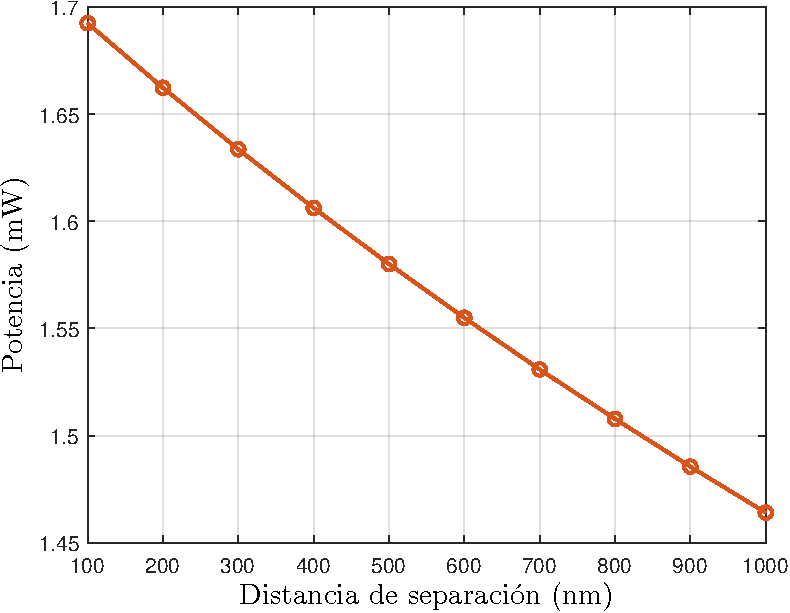
\includegraphics[width=0.6\textwidth]{figuras/Resultados/conduccion/pdf/Prc_SiCSiO2Ge.pdf}
	\caption{ }
	\label{fig:Prc_SiCSiO2Ge}
\end{figure}

\begin{figure}[H]
	\centering
	%% Si-SiO2-Si Eg
	\begin{subfigure}[b]{0.49\textwidth}
		\centering
		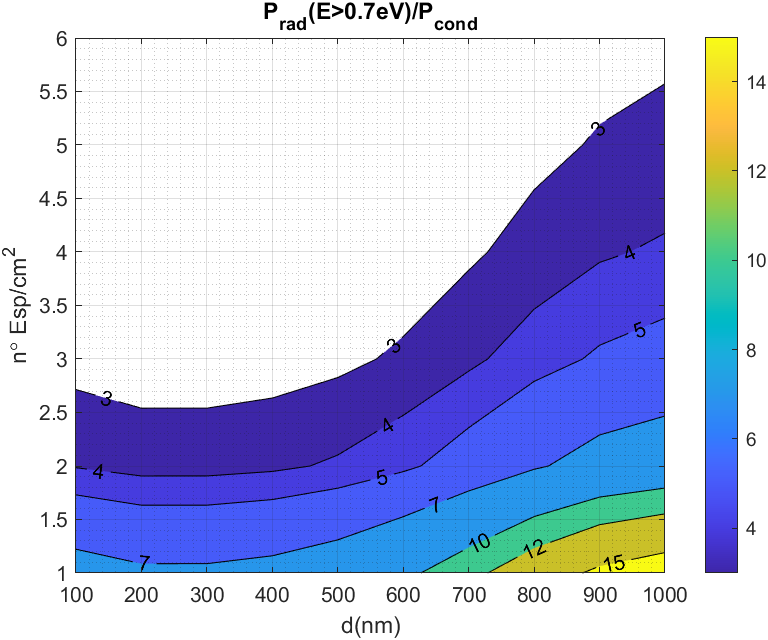
\includegraphics[width=1.00\textwidth]{figuras/Resultados/RelacionCondRad/SiC_Ge.png}
		\caption{ }
		\label{fig:rel_SiCSiO2Ge}
	\end{subfigure}
	\hfill
	\begin{subfigure}[b]{0.49\textwidth}
		\centering
		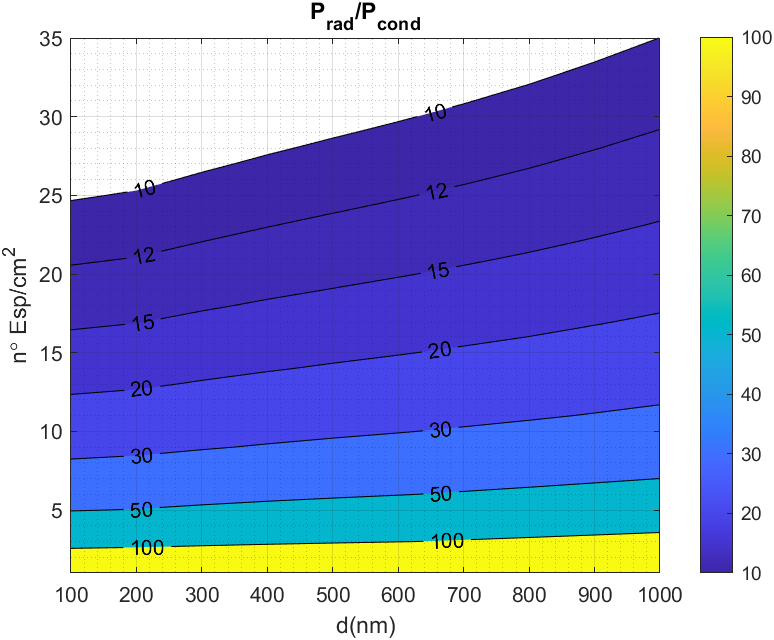
\includegraphics[width=1.00\textwidth]{figuras/Resultados/RelacionCondRad/SiC_Ge_full.png}
		\caption{ }
		\label{fig:rel_SiCSiO2Ge_Rc}
	\end{subfigure}
	\hfill
	\begin{subfigure}[b]{0.49\textwidth}
		\centering
		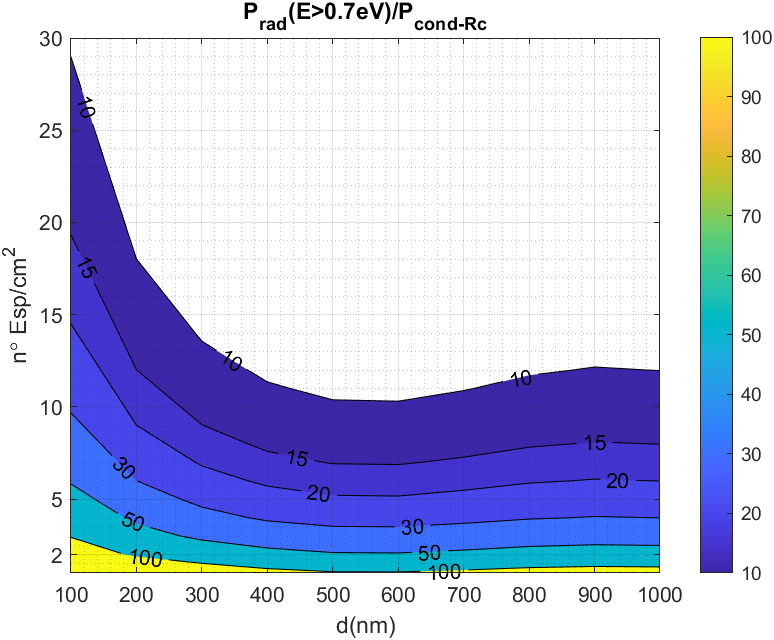
\includegraphics[width=1.00\textwidth]{figuras/Resultados/RelacionCondRad/SiC_Rc.png}
		\caption{ }
		\label{fig:rel_SiCSiO2Ge_full}
	\end{subfigure}
	\hfill
	\begin{subfigure}[b]{0.49\textwidth}
		\centering
		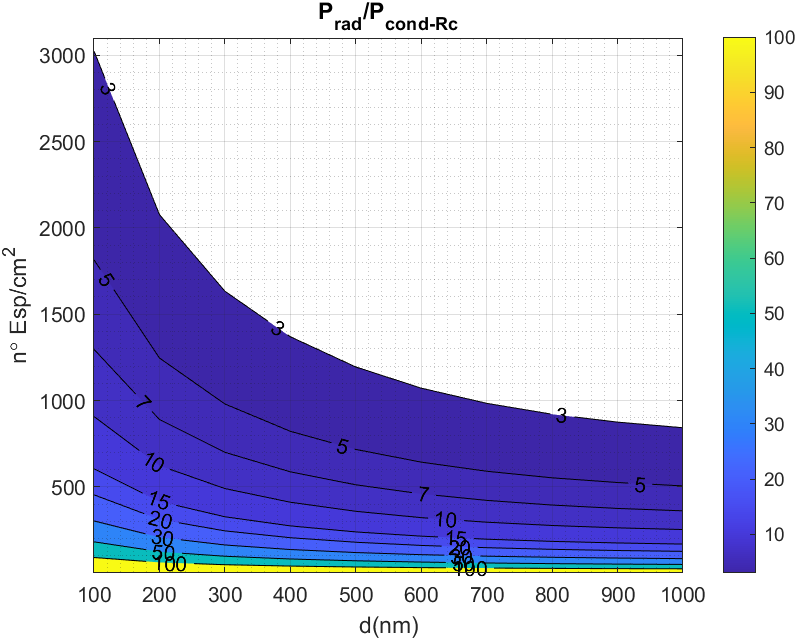
\includegraphics[width=1.00\textwidth]{figuras/Resultados/RelacionCondRad/SiC_Ge_Rc_full.png}
		\caption{ }
		\label{fig:rel_SiCSiO2Ge_Rc_full}
	\end{subfigure}
	\caption{ }
	\label{fig:relation_SiCSiO2Ge}
\end{figure}

\section{Resultados de las simulaciones para una TPV de Si-Si-Ge y SS-Si-Ge}
%% comparar el efecto de cambiar el material del nano-espaciador
\begin{table}[H]
	\centering
		\begin{tabular}{|c|c|c|}
		\hline
		dnm&Prcpaper&Prc\_SS\\ \hline 
		100&0,0017136&0,00171126\\ \hline 
		200&0,0017135&0,00171117\\ \hline 
		300&0,00171336&0,00171103\\ \hline 
		400&0,00171322&0,00171089\\ \hline 
		500&0,00171304&0,00171072\\ \hline 
		600&0,00171282&0,0017105\\ \hline 
		700&0,00171257&0,00171025\\ \hline 
		800&0,0017125&0,00171019\\ \hline 
		900&0,0017122&0,00170989\\ \hline 
		1000&0,00171208&0,00170978\\ \hline
		\end{tabular}
	\caption{nano-espaciador de Si}
	\label{tab:nanoEspaciadorDeSi}
\end{table}
\begin{figure}[H]
	\centering
		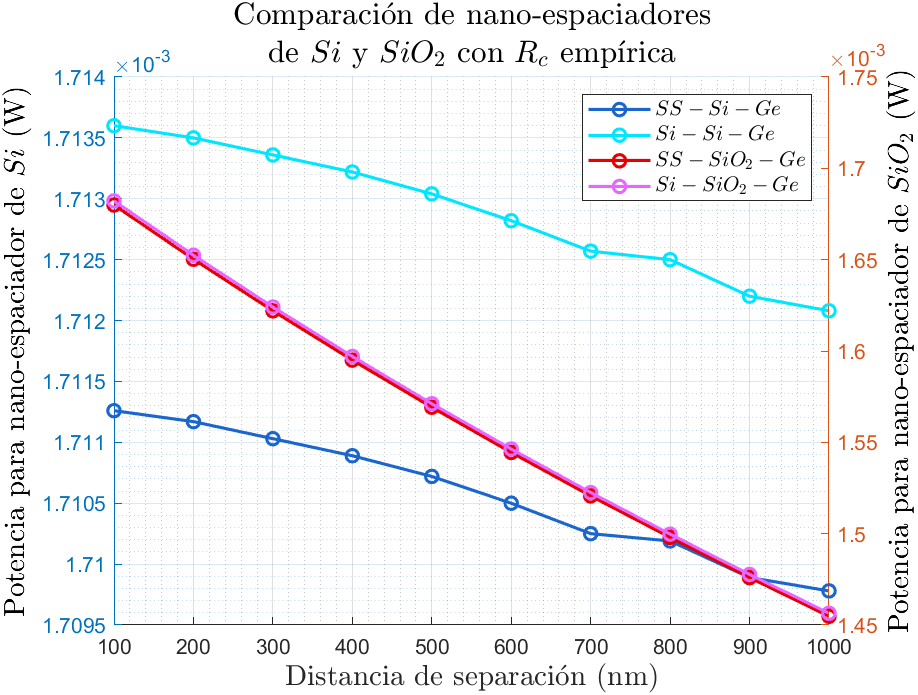
\includegraphics[width=0.6\textwidth]{figuras/Resultados/conduccion/relaciones_SiySiO2.png}
	\caption{ }
	\label{fig:relaciones_SiySiO2}
\end{figure}

\section{Discusión}